% Este documento destina-se a servir como modelo para a produção de documentos
% de pesquisa do PPGINF/UFPR, como projetos, dissertações e teses. A classe de
% documento se chama "ppginf" (arquivo ppginf.cls) e define o formato básico do
% documento. O texto está organizado em capítulos que são colocados em
% subdiretórios separados. São definidos exemplos para a inclusão de figuras,
% códigos-fonte e a definição de tabelas.
%
% Produzido por Carlos Maziero (maziero@inf.ufpr.br) em Outubro de 2015.
% Adaptado de um modelo anterior construído pelo autor para o PPGIA/PUCPR.

% Opções da classe ppginf:
% - defesa: espaçamento 1,5, sem algumas páginas iniciais (default)
% - final:  espaçamento simples, completa
% - oneside: para impressão somente frente (default)
% - twoside: para impressão frente/verso
% - ... (demais opções aceitas pela classe "book")

% Opções default: defesa, oneside
\PassOptionsToPackage{table,xcdraw}{xcolor}
\documentclass[defesa,oneside]{ppginf}
%\documentclass[final,twoside]{ppginf}

% configurações de diversos pacotes, inclusive o fonte principal do texto
% Pacotes usados neste documento e suas respectivas configurações

% seleção de línguas do texto (a última é a principal/default)
\usepackage[english,brazilian]{babel}

% ------------------------------------------------------------------------------
% Definição de fontes

% formato dos arquivos-fonte (utf8 no Linux e latin1 no Windows)
\usepackage[utf8]{inputenc}	% arquivos LaTeX em Unicode (UTF8)

% usar codificação T1 para ter caracteres acentuados corretos no PDF
\usepackage[T1]{fontenc}

% fonte usada no corpo do texto (descomente apenas uma)
\usepackage{newtxtext,newtxmath}	% Times (se não tiver, use mathptmx)
%\usepackage{lmodern}			% Computer Modern (fonte clássico LaTeX)
%\usepackage{kpfonts}			% Kepler/Palatino (idem, use mathpazo)
%\renewcommand{\familydefault}{\sfdefault} % Arial/Helvética (leia abaixo)

% A biblioteca central da UFPR recomenda usar Arial, seguindo a recomendação da
% ABNT. Essa é uma escolha ruim, pois fontes sans-serif são geralmente inade-
% quados para textos longos e impressos, sendo melhores para páginas Web.
% http://www.webdesignerdepot.com/2013/03/serif-vs-sans-the-final-battle/.

% fontes usadas em ambientes específicos
\usepackage[scaled=0.9]{helvet}		% Sans Serif
\usepackage{courier}			% Verbatim, Listings, etc

% ------------------------------------------------------------------------------

% inclusão de figuras
\usepackage{graphicx}			% incluir figuras em PDF, PNG, PS, EPS

% subfiguras (subfigure is deprecated, don't use it)
\usepackage[labelformat=simple]{subcaption}
\renewcommand\thesubfigure{(\alph{subfigure})}

% ------------------------------------------------------------------------------

% inclusão/formatação de código-fonte (programas)
\usepackage{listings}
\lstset{language=c}
\lstset{basicstyle=\ttfamily\footnotesize,commentstyle=\textit,stringstyle=\ttfamily}
\lstset{showspaces=false,showtabs=false,showstringspaces=false}
\lstset{numbers=left,stepnumber=1,numberstyle=\tiny}
\lstset{columns=flexible,mathescape=true}
\lstset{frame=single}
\lstset{inputencoding=utf8,extendedchars=true}
\lstset{literate={á}{{\'a}}1  {ã}{{\~a}}1 {à}{{\`a}}1 {â}{{\^a}}1
                 {Á}{{\'A}}1  {Ã}{{\~A}}1 {À}{{\`A}}1 {Â}{{\^A}}1
                 {é}{{\'e}}1  {ê}{{\^e}}1 {É}{{\'E}}1  {Ê}{{\^E}}1
                 {í}{{\'\i}}1 {Í}{{\'I}}1
                 {ó}{{\'o}}1  {õ}{{\~o}}1 {ô}{{\^o}}1
                 {Ó}{{\'O}}1  {Õ}{{\~O}}1 {Ô}{{\^O}}1
                 {ú}{{\'u}}1  {Ú}{{\'U}}1
                 {ç}{{\c{c}}}1 {Ç}{{\c{C}}}1 }

% formatação de algoritmos
\usepackage{algpseudocode,algorithm,algorithmicx}
\floatname{algorithm}{Algoritmo}
\renewcommand{\algorithmiccomment}[1]{~~~// #1}
%\algsetup{linenosize=\footnotesize,linenodelimiter=.}

% ------------------------------------------------------------------------------

% outros pacotes
\usepackage{alltt,moreverb}	% mais comandos no modo verbatim
\usepackage{lipsum}		% gera texto aleatório (para os exemplos)
\usepackage{currfile}		% infos sobre o arquivo/diretório atual
\usepackage[final]{pdfpages}	% inclusão de páginas em PDF
\usepackage{longtable}		% tabelas multi-páginas (tab símbolos/acrônimos)

% listas de símbolos e de abreviações (a fazer)
%\usepackage[titles]{tocloft}
%\newlistof[part]{symb}{los}{Lista de Símbolos}
%\newlistof[part]{abbrev}{loa}{Lista de Abreviações}
%\newcommand{\symb}[2]{%
%\refstepcounter{symb}
%\addcontentsline{los}{symb}{\protect #1 :#2}\par}








%=====================================================

\begin {document}

% Principais dados, usados para gerar as páginas iniciais.
% Campos não utilizados podem ser removidos ou comentados.

\title{Meta-Heurísticas e Hiper-Heurísticas  aplicadas ao problema de dobramento de proteínas}

% Estas devem ser definidas aqui para poder incorporar nos metadados do PDF
\pchave{palavra-chave 1, palavra-chave 2, palavra-chave 3}
\keyword{keyword 1, keyword 2, keyword 3}

\author{Vidal Daniel da Fontoura}
\advisor{Aurora Trinidad Ramirez Pozo}
\coadvisor{Roberto Santana }

\field{Ciência da Computação}		% default do PPGInf, não mudar

\date{2016}
\local{Curitiba PR}
\instit{UFPR}{Universidade Federal do Paraná}

%% Descrição do documento (obviamente, descomentar somente UMA!)

%\descr{Tese apresentada como requisito parcial à obtenção do grau de Doutor em Informática no Programa de Pós-Graduação em Informática, setor de Ciências Exatas, da Universidade Federal do Paraná}

%\descr{Documento apresentado como requisito parcial para o exame de qualificação de Doutorado no Programa de Pós-Graduação em Informática, setor de Ciências Exatas, da Universidade Federal do Paraná}

\descr{Dissertação apresentada como requisito parcial à obtenção do grau de Mestre em Informática no Programa de Pós-Graduação em Informática, setor de Ciências Exatas, da Universidade Federal do Paraná}

%\descr{Documento apresentado como requisito parcial para o exame de qualificação de Mestrado no Programa de Pós-Graduação em Informática, setor de Ciências Exatas, da Universidade Federal do Paraná}

%\descr{Trabalho apresentado como requisito parcial à conclusão do Curso de Bacharelado em XYZ, setor de Ciências Exatas, da Universidade Federal do Paraná}

%\descr{Trabalho apresentado como requisito parcial à conclusão da disciplina XYZ no Curso de Bacharelado em XYZ, setor de Ciências Exatas, da Universidade Federal do Paraná}

%=====================================================

% páginas iniciais (preâmbulo)
\frontmatter
\pagestyle{frontmatter}

% capa e folha de rosto
\titlepage

% páginas que só aparecem na versão final (inclusão automática)
% - IMPORTANTE - IMPORTANTE - IMPORTANTE - IMPORTANTE -
%
% O conteúdo exato da ficha catalográfica é preparada pela Biblioteca Central
% da UFPR, a pedido da secretaria do PPGINF. Não "invente" um conteúdo para ela,
% se informe a respeito com nossa secretária.

\begin{ficha}	% só gera conteúdo se for na versão final

% "Ficha" provisória (comentar quando tiver a ficha oficial)
\begin{center}
\textbf{Ficha Catalográfica}

~

\emph{Esta folha deve ser substituída pela ficha catalográfica fornecida pela Biblioteca Central da UFPR, a pedido da secretaria do PPGInf/UFPR (vide arquivo \texttt{ficha.tex}).}
\end{center}

% para a inclusão da ficha catalográfica final em formato PDF
%\includepdf[\thispagestyle{empty},noautoscale]{ficha.pdf}

\end{ficha}

%=====================================================
		% ficha catalográfica
% A ficha de aprovação será fornecida pela secretaria do programa,
% após a defesa e cumprimento dos demais trâmites legais.

\begin{aprovacao}	% só gera conteúdo se for na versão final

% "Texto" provisório (remover quando tiver a aprovacao oficial)
\begin{center}
\textbf{Termo de aprovação}

~

\emph{Esta folha deve ser substituída pela ata de defesa ou termo de aprovação devidamente assinado, que será fornecido pela secretaria do programa após a defesa ter sido concluída e aprovada (vide arquivo \texttt{aprovacao.tex}).}
\end{center}

% para a inclusão da aprovacao final em formato PDF:
%\includepdf[\thispagestyle{empty},noautoscale]{aprovacao.pdf}

\end{aprovacao}

%=====================================================
		% folha de aprovação
\begin{dedica}  % só gera conteúdo se for na versão final

A alguém...

\end{dedica}

		% dedicatória
\begin{agradece}	% só gera conteúdo se for na versão final

Inserir os agradecimentos. Os agradecimentos devem ocupar no máximo uma página, devem ser justificados na largura da página e com um afastamento de parágrafo na primeira linha de 1,27 cm. O espaçamento entre linhas deve ser de 1,5 linhas. Não deve haver espaçamento adicional entre parágrafos.

\lipsum[2-5]	% gera um texto aleatório

\end{agradece}

		% agradecimentos

% resumo e abstract
\begin{resumo}


Proteínas são estruturas, compostas por aminoácidos, que exercem um papel importante na natureza. Estas estruturas são formadas a partir de um processo de dobramento, no qual uma sequência de aminoácidos inicialmente desdobrada irá adotar uma conformação/estrutura espacial única/nativa. Entretanto, o processo de dobramento ainda não é completamente compreendido e é considerado um dos maiores desafios das áreas de biologia, química, medicina e bioinformática. Este desafio é conhecido como o problema de dobramento de proteínas (PDP) e trata da predição de estruturas de proteínas. 

O PDP pode ser visto como um problema de minimização, pois é afirmado que a estrutura nativa de uma proteína é aquela que minimiza sua energia global livre. Dessa maneira, diversas estudos aplicam estratégias heurísticas para explorar modelos simplificados. tais como o modelo HP. Embora simplificado, o modelo HP possui um complexo espaço de busca com muitos mínimos locais.  

%todo precisar arrumar essa fita aqui VIDAL citar grande variabilidade entre as instnacias

 Se trata de um problema complexo com muitos mínimos locais e com grande variabilidade nas características entre diferente. instâncias. Dessa maneira surge a demanda de estratégias que possuam mecanismos robustos para explorar de maneira adequadaca o espaço de busca. É nesse contexto que hiper-heurísticas se apresentam como boas opções para explorar o espaço de busca de problemas complexos. 



Nesta dissertação, são apresentadas duas abordagens para o PDP. A primeira visa a aplicação de algoritmos evolucionários multi objetivos para resolver o PDP. A segunda consiste no \textit{design} automático de heurísticas de alto nível utilizando uma técnica de programação genética chamada evolução gramatical, a qual utiliza uma gramática para produzir programas de computador. 

 As estratégias propostas foram aplicadas utilizando um conjunto de \text{benchmark} com diferentes sequências de aminoácidos. Os resultados foram comparados com outros trabalhos que utilizam o mesmo conjunto de \textit{benchmark}. Alguns resultados obtidos se mostraram promissores dessa maneira motivando novos estudos que visem estratégias adaptativas para o PDP.



\end{resumo}


\begin{otherlanguage}{english}

\begin{abstract}

% em inglês, o primeiro parágrafo não deve ser indentado
\noindent

Proteins are structures composed by amino acids that plays a important role in nature. These structures are built by a process called protein folding, where a sequence of amino-acids initially unfolded will obtain your native structure. However, the protein folding process is not entire understood and it is considered one of the most challenging problem from biology, chemistry, medicine and bio-informatics. This problem is knows as the protein folding problem (PFP) and handles the prediction of protein structures.

The PFP is a minimization problem, because the proteins native structures are the one within minimum energy. Thus, many heuristics strategies make use of simplified models, such as the HP model, to find the proteins native structures within the HP model. Although simplified, the HP model has a complex search space and a great variability of characteristics between the instances. Thus, raises the demand of strategies with robust mechanisms to explore the search space properly. In this context, adaptive strategies fits well as good alternative to explore the fitness landscape from complex problems.
 
 In this dissertation, two approaches are presented to solve the PDP. The first one describes a bi objective approach applying traditional multi objective evolutionary algorithms. The second approach consists the automated design of high level heuristics using a genetic programming technique called grammatical evolution, which uses a grammar to produce computer programs.  

Both approaches proposed have been applied on a benchmark set with different amino acids sequences. The results have been compared with previous studies that used the same benchmark. In some cases the results obtained are promising which motivates the development of new adaptive strategies to solve the PFP.  


\end{abstract}

\end{otherlanguage}



% sumário e demais listas (figuras, tabelas, abreviações/siglas, símbolos)
\tableofcontents
\listoffigures
\listoftables
%=====================================================

% lista de acrônimos (siglas e abreviações)

\begin{listaacron}

\begin{longtable}{ll}
DINF & Departamento de Informática\\
PPGINF & Programa de Pós-Graduação em Informática\\
UFPR & Universidade Federal do Paraná\\
\end{longtable}

\end{listaacron}

%=====================================================
		% ainda deve ser preenchida à mão
%=====================================================

% lista de símbolos

\begin{listasimb}

\begin{longtable}{ll}
$RC$ & \textit{Reward Credit}, crédito obtido.\\
$C_{best}$ & \textit{Current Best Solution}, melhor solução atual.\\
$C_{current}$ & \textit{Current Solution}, solução atual\\
$C_{accept}$ & \textit{Current Solution Accpted}, vezes que a solução atual foi aceita.\\
$C_{ava}$ & \textit{Average Reward Credit}, média de créditos obtidos anteriormente. \\
$C_r$ & \textit{Times Ranked First} número de vezes classificada como primeiras.\\

$Delta$ & \textit{Fitness Difference}, a diferença de qualidade\\
 $PF$ & \textit{Previous Fitness}, a qualidade da solução anterior.\\
 $CF$ & \textit{Current Fitness}, a qualidade da solução atual.\\
 
 $CI$ & \textit{Current Iteraction}, iteração corrente.\\
 $TI$ & \textit{Total Number of Iteractions}, número total de iterações.

\end{longtable}

\end{listasimb}

%=====================================================
		% idem

%=====================================================

% corpo do documento
\mainmatter
\pagestyle{mainmatter}

% inclusao de cada capítulo, alterar a gosto (do professor de Metodologia...)
\chapter{Introdução}

As proteínas são responsáveis por muitas funções importantes das células vivas. Estas estruturas garantem o correto funcionamento de um amplo número de entidades biológicas. As proteínas são o produto de um processo chamado de dobramento de proteínas, no qual uma cadeia de aminoácidos inicialmente desdobrada será transformada em sua estrutura final/nativa. A predição de estruturas de proteínas possui um campo amplo de aplicações biotecnológicas e médicas. Por exemplo: síntese de novas proteínas e dobramentos \cite{wang2012structural, rothlisberger2008kemp}, síntese de novas drogas baseada nas estruturas \cite{qian2004improvement, krieger2009improving}  e obtenção experimental de estruturas a partir de dados incompletos de ressonância magnética nuclear \cite{shen2009novo}.  

Determinar a estrutura nativa de proteínas é uma tarefa desafiadora até mesmo para super computadores modernos. Isto ocorre por conta do imenso espaço de busca para avaliar todas as possíveis configurações que uma dada proteína pode adotar. Diferentes formas de representar as estruturas/conformações de proteínas existem e podem ser utilizadas para simular o processo de dobramento. Embora existam modelos extremamente detalhados, estas representações são computacionalmente muito custosas \cite{benitez2015algoritmo, santana2008protein}. Consequentemente, muitos autores \cite{custodio2004investigation,hsu2003growth,lin2011protein,unger1993genetic,santanna2008,custodio2014multiple, garza2012locality} utilizam modelos simplificados para representar as estruturas de proteínas. Um modelo bastante conhecido para este propósito, criado por Lau and Dill \cite{lau1989lattice}, é o modelo Hidrofóbico-Polar (HP). Este modelo simplifica os aminoácidos em apenas dois tipos: hidrofóbico (H) e polar (P). 

Para avaliar as estruturas representadas pelo modelo HP é preciso computar o valor de energia associado a uma dada conformação \cite{unger1993genetic}. Para isto, é necessário considerar as interações entre os aminoácidos. Uma interação ocorre quando o par de aminoácidos é adjacente no \textit{grid}/cubo e não é adjacente na sequência. No modelo HP existem apenas três tipos: HP, HH e PP. Porém somente interações hidrofóbicas (HH) influenciam no valor de energia referente a uma conformação \cite{unger1993genetic}. A questão que surge é como buscar, dentre as possíveis conformações, aquela cuja energia seja mínima. Embora, o modelo HP seja um modelo simplificado este se apresenta como um problema NP-Completo e as instâncias apresentam uma grande variabilidade entre si. Dessa maneira, é muito difícil um algoritmo encontrar a conformação ótima. Outra dificuldade encontrada por pesquisadores é a configuração dos parâmetros para os algoritmos. Esta tarefa costuma tomar muito tempo pois a melhor maneira de encontrar a configuração ideal é por tentativa e erro.

É nesse contexto que as hiper-heurísticas e estratégias adaptativas, tais como utilizar operadores genéticos de maneira dinâmica, geralmente são aplicadas e vem apresentando bons resultados \cite{burke2013hyper}. Entretanto, não existem muitas abordagens que visam o projeto automático de novas heurísticas ou automatização da seleção de heurísticas existentes para o PDP. Assim como a maioria dos trabalhos tratam o PDP de maneira mono objetiva. Consequentemente, existem poucos trabalhos que propõem estratégias multi objetivas.

Esta dissertação apresenta duas abordagens para o PDP. A primeira trata-se de uma estratégia multi objetiva para o PDP utilizando algoritmos evolucionários multi objetivos (AEMOs) do estado da arte. Este estudo \cite{fontouralimacbic2015} foi publicado no XII CBIC - Congresso Brasileiro de Inteligência Computacional. Posteriormente este estudo foi estendido para compor o livro \textit{Evolutionary Multi-Objective System Designs} o qual está sendo produzido. Duas adaptações foram propostas para os AEMOs com objetivo de melhorar os resultados obtidos. Já a segunda abordagem consiste em uma estratégia de projeto automático de heurísticas de alto nível para um \textit{framework} hiper heurístico.




\section{Organização do Texto}
\label{Introducao:Organizacao do Texto}

O restante desta dissertação está organizado da seguinte maneira: no capítulo \ref{cap:pdp} é introduzido o referencial teórico necessário para uma boa compreensão sobre o PDP. Já no capítulo \ref{cap:Referencial Teórico} são apresentados conceitos relacionados com os AEMOs, assim como os algoritmos que foram utilizados nesta dissertação. Ainda são discutidos os aspectos referentes as hiper-heurísticas, sua classificação e também conceitos de programação genética (PG) e evolução gramatical (EG). Em seguida, o capítulo \ref{cap:Trabalhos Relacionados} apresenta estudos relacionados com esta dissertação. A duas abordagens propostas são apresentadas no capítulo \ref{cap:Metodologia}. Os experimentos realizados com as duas abordagens são apresentados no capítulo \ref{cap:experimentos}. Finalmente, o capítulo \ref{cap:conclusao} apresenta a conclusão desta dissertação.







 			% introdução
\chapter{Problema de Dobramento de Proteínas}
\label{cap:pdp}

% figuras estão no subdiretório "figuras/" dentro deste Capítulo
\graphicspath{\currfiledir/figuras/}

%=====================================================

\section{PDP - Problema de Dobramento de Proteínas}
\label{sec:ProblemaDobramentoProteínas}

Proteínas são estruturas básicas, essenciais para vida e possuem incontáveis funções biológicas. Proteínas são sintetizadas pelos ribossomos seguindo um formato provido pelo mensageiro RNA (mRNA). Durante a síntese, as proteínas dobram (enovelam) em uma estrutura tridimensional única, conhecida como conformação nativa. Este processo é chamado de dobramento de proteínas (\textit{protein folding}). A função biológica de uma proteína depende da sua estrutura tridimensional \cite{unger1993genetic}.

As proteínas são polímeros compostos por sequências de aminoácidos (também chamados de resíduos) conectados linearmente por ligações peptídicas. Cada aminoácido é composto por um átomo central de carbono ($C\alpha$) conectado a um átomo de hidrogênio, um grupo amina, um grupo carboxila e uma cadeia lateral (\textit{side-chain}) a qual confere a cada aminoácido uma função distinta. Uma ligação peptídica é formada por dois aminoácidos quando o grupo carboxila de uma molécula reage com o grupo amina da outra. Este processo de agregação de aminoácidos é conhecido como desidratação pois libera uma molécula de água ($H_2O$) \cite{suzuki1986introduction}. Proteínas podem ser chamadas de cadeias polipeptídicas. Todos os aminoácidos tem a mesma cadeia principal (\textit{backbone}) e se diferem dos outros apenas pela cadeia lateral (\textit{side-chain}), a qual pode ser um simples átomo de hidrogênio ou até um grupo heterocíclico complexo. A \textit{side-chain} define as propriedades físicas e químicas dos aminoácidos de uma proteína \cite{cox2013lehninger}.

%\subsection{Estrutura hierárquica e função das proteínas}

%As proteínas são tradicionalmente descritas em quatro níveis hierárquicos de %complexidade \cite{cox2013lehninger}:

%\begin{enumerate}
%	\item Estrutura primária: Nível de organização simples que visa representar apenas a sequência de aminoácidos de maneira linear. Representa apenas as ligações peptídicas entre os aminoácidos. (Colocar imagem?)
%	\item Estrutura secundária: Consiste em arranjos espaciais de regiões locais de uma proteína. Existem três estruturas secundárias importantes $\alpha$-hélices(PAULING; COREY; BRANSON, 1951a), $\beta$-folhas
%	(PAULING; COREY; BRANSON, 1951b) e turns (dobras) (LEWIS; MOMANY;
%	SCHERAGA, 1973).
%	$\alpha$-hélices é a forma mais comum de estrutura secundária. É uma estrutura semelhante a um bastão, onde o \textit{backbone} firmemente 
%	helicoide forma a parte interna do bastão, e as \textit{side-chains} se projetam para fora em uma disposição helicoidal(http://labs.icb.ufmg.br/lbcd/grupo1/alfa.html). $\beta$-folhas formada por 2 ou mais segmentos polipeptídicos da mesma molécula, ou de moléculas diferentes, dispostos lateralmente e estabilizados por pontes de hidrogênio entre os grupos $NH$ e $CO$.  (Benítez)
%	\textit{Turns} são compostos de três ou quatro aminoácidos e geralmente são localizados na superfície das proteínas formando dobras que redirecionam a cadeia polipeptídica para o interior da proteína. \textit{Turns} permitem que as proteínas sejam dobradas em estruturas altamente compactas.	As estruturas secundárias podem ser associadas formando estruturas super secundárias, chamadas de \textit{motifs} (BRANDEN; TOOZE, 1999; GRIFFITHS
%	et al., 2000; NÖLTING, 2006). Os \textit{motifs}  são padrões frequentemente encontrados em estruturas tridimensionais.
%\item Estrutura terciária: Trata do arranjo tridimensional dos aminoácidos que compõem uma proteína. Enquanto as estruturas secundárias são estabilizadas por pontes de hidrogênio, as estruturas terciárias são estabilizadas por iterações entre \textit{side-chains} hidrofóbicas e pontes de hidrogênio entre \textit{side-chains} polares. A estrutura terciária representa o dobramento de um polipeptídeo como resultado das interações entre as \textit{side-chains} dos aminoácidos que se encontram em diferentes regiões da estrutura primária.
%	\item Estrutura quaternária: É o nível de representação mais complexo e descreve o arranjo de duas mais subunidades polipeptídicas dobradas (estruturas terciárias) no espaço.
%A associação quaternária pode ser entre diferentes tipos de polipeptídeos (heterodímero)
%ou entre polipeptídeos idênticos (homodímero). Este nível de organização	descreve o número e posições relativas de subunidades em proteínas
%multiméricas. A Hemoglobina é um exemplo de proteína multimérica, pois é composta de duas cópias de polipeptídeos diferentes que interagem entre si. 

%\end{enumerate}

\section{Dobramento de proteínas}

É o processo em que cada cadeia polipeptídica é transformada em uma estrutura compacta que realiza alguma função biológica \cite{grantcharova2001mechanisms}. Estas funções incluem controle e regulação de processos químicos essenciais para os organismos vivos \cite{branden1999introduction}. A estrutura tridimensional mais estável é chamada de conformação nativa e é a qual permite que a proteína exerça corretamente sua função biológica \cite{lodish2000molecular, pedersen2000algorithms}.

Experimentos conduzidos por Anfinsen et al. \cite{sela1957reductive, anfinsen1972studies, anfinsen1961kinetics}, mostraram que as proteínas possuem apenas uma conformação nativa e que as informações essenciais que codificam a estrutura estão contidas na sequência de aminoácidos. A conformação tridimensional nativa é dada pela estrutura primária (sequência de aminoácidos) de uma proteína.

Muitas proteínas podem desnaturar por modificações no ambiente em que estão inseridas, conforme demonstrado por \cite{sela1957reductive, anfinsen1972studies, anfinsen1961kinetics}. Durante o processo de desnaturação as proteínas perdem sua forma nativa (desdobram) e, consequentemente, perdem sua função. O exemplo mais conhecido de desnaturação proteica é o da clara do ovo. A clara do ovo é composta por água e albumina. A albumina é uma proteína polar, portanto solúvel em 
água. Ao fritar ou cozinhar o ovo, eleva-se a temperatura, levando à desnaturação da albumina que, mesmo ao retornar à temperatura original, não consegue voltar à sua conformação nativa. Além de se desdobrarem é possível que ocorram erros de dobramento na formação das proteínas causando com que a proteína não exerça sua função biológica corretamente. Estudos tentam identificar causas para os erros de dobramento das proteínas pois, muitas enfermidades são causadas por conta disto, por exemplo, mal de Alzheimer \cite{hutton2001analysis, selkoe2001clearing}, alguns tipos de câncer \cite{bell2002p53, dawson2003n, ishimaru2003fibrillar}, fibrose cística \cite{thomas1992altered}, arteriosclerose
\cite{ursini2002atherosclerosis}, mal de Parkinson \cite{mcnaught2001failure}, entre outras. 
Portanto, entender como o processo de dobramento de proteínas ocorre é de fundamental importância. 

Um dos objetivos comuns das ciências biológicas é caracterizar funcionalmente sequências de proteínas através da resolução de suas conformações nativas \cite{eswar2003tools}. Varias áreas da ciência, tais como Biologia, Medicina, Química Orgânica, realizam diferentes estudos das proteínas. Muitos destes estudos são voltados para o processo de dobramento das proteínas que pode sofrer alterações: tanto em como a conformação estará disposta no espaço, como ela estará agrupada e sobre sua má formação. Isto é muito relevante para estudos que visam à produção de medicamentos, suplementos alimentares, técnicas que manipulam o DNA, ou para formação de novos compostos proteicos sintéticos em laboratório \cite{devlin1998manual}. É importante mencionar que apesar do avanço na grande quantidade de proteínas que se tem conhecimento por conta de projetos de sequenciamento genômico, apenas uma pequena fração de estruturas tridimensionais é conhecida.

A cristalografia de raios-X e espectroscopia de RNM são os métodos experimentais mais poderosos para o estudo da estruturas de proteínas \cite{ilari2008protein} \cite{gobl2012application}. Entretanto estes métodos são altamente custosos tanto em esforços computacionais, de tempo e financeiros, e estão disponíveis apenas para algumas instituições.


Embora o conceito de dobramento de proteínas tenha surgido da área de biologia molecular, este problema é um tópico interdisciplinar, o qual requer apoio de muitas áreas do conhecimento, e é considerado como um dos desafios atuais mais importantes da biologia e bioinformática \cite{nicosia2008generalized}. 

Na biologia computacional existem dois problemas que tratam sobre o dobramento de proteínas. São eles: problema de predição estrutura de proteínas (ou PSP - \textit{Protein Structure Prediction}), que trata de predizer a estrutura tridimensional (conformação) a partir de sua sequência (estrutura primária); e o problema de dobramento de proteínas (PDP ou PFP - \textit{Protein Folding Problem}), o qual trata da determinação dos passos/eventos que conduzem o dobramento a partir da estrutura primária até a conformação nativa \cite{lopes2008evolutionary}. Porém, na literatura, são encontrado ambos os termos sendo utilizados sem nenhuma distinção, normalmente se referindo apenas ao primeiro problema \cite{lopes2008evolutionary}.  

A ciência da computação desempenha um papel importante nisto, propondo e desenvolvendo modelos e soluções computacionais para o estudo de ambos os problemas PSP e PDP \cite{lopes2008evolutionary}. Muitas estratégias computacionais descrevem modelos de predição para estruturas proteicas com diferentes níveis de detalhamento e complexidade. Embora, existam modelos com um elevado grau de detalhamento simular a predição de estruturas das proteínas é computacionalmente muito custosa. É nesta lacuna que se abre espaço para estratégias que proponham modelos simplificados para representar estruturas de proteínas sem perda de viabilidade computacional \cite{benitez2015algoritmo}. Consequentemente, é possível evitar a obrigatoriedade de métodos caros e assim aumentar a capacidade de centros de pesquisa, com recursos escassos, desenvolverem abordagens com modelos simplificados para representar as estruturas. Apesar de complexidade reduzida estes modelos apresentam uma maneira fidedigna de representar as estruturas de proteínas. 


Segundo a lei da termodinâmica \cite{anfinsen1972studies}, a estrutura de uma proteína se torna estável quando adquire o seu estado nativo, em qual a sua energia livre é mínima. Os modelos de predição de estruturas normalmente são baseados nesta lei. Dessa maneira, o problema é modelado com objetivo de minimizar energia livre das possíveis conformações que uma proteína pode assumir \cite{benitez2015algoritmo}. Estes modelos assumem que o principal fator para formação das estruturas de proteínas segue a lei da termodinâmica. Portanto, a conformação nativa de uma proteína é dada por aquela que possuir o menor valor de energia livre.

\cite{pedersen2000algorithms} sugere que um modelo computacional deve possuir algumas características:

\begin{itemize}
	\item Um conjunto de entidades que representam os átomos e as ligações entre eles. 
	\item Regras que definem as possíveis conformações.
	\item Uma função que seja computacionalmente factível para calcular a energia livre das possíveis conformações.
\end{itemize}

A próxima subseção irá discorrer sobre alguns modelos para representar as estruturas de proteínas.

\section{Modelos de Representação de Proteínas}

Em suma, existem duas classes de modelos de representação de estruturas de proteínas: analítico (também conhecido como \textit{all atom}) e discreto (chamado também de \textit{coarse-grained}). Os modelos analíticos possuem uma descrição detalhada da estrutura tridimensional incluindo informações de todos os átomos que constituem uma proteína. Já os modelos discretos descrevem as proteínas com um nível bastante reduzido de detalhes. Recentemente, os modelos discretos ganharam maior interesse, por conta de dois fatores \cite{benitez2015algoritmo}:

\begin{itemize}
	\item A simulação de modelos analíticos nem sempre é computacionalmente possível por conta do alto custo envolvido.
	\item Modelos discretos possibilitam simulações biologicamente relevantes com melhor aproveitamento  computacional . 
	
\end{itemize}

 Nesta dissertação, são descritos apenas os modelos discretos pois visa a utilização do modelo hidrofóbico polar (HP) 2D.

\subsection{Modelos Discretos}

Os modelos computacionais mais simples são os conhecidos como modelos de grade (\textit{lattice models}). Estes modelos consideram as estruturas de proteínas como um colar de esferas posicionado em uma grade. O grau de liberdade dos movimentos é restrito à estrutura da grade, que pode ser 2D (plano) ou 3D (espacial). Conformações válidas são aquelas que os aminoácidos adjacentes na sequência também são adjacentes na grade e cada aminoácido ocupe uma posição distinta na grade. Muitos modelos de grade têm sido propostos e aplicados ao PDP. Os modelos 2D-HP e 3D-HP são exemplos de modelos de grade.

\subsubsection{Modelo Hidrofóbico-Polar (HP)}
\label{subsubsection:modeloHP}

No modelo HP os aminoácidos são classificados em 2 tipos: Hidrofílicos (Polar) e Hidrofóbico. Consequentemente, uma proteína é representada por uma \textit{string} de caracteres definida por um alfabeto binário $\{H,P\}$. Este modelo considera que as interações entre aminoácidos hidrofóbicos (H) representam a contribuição mais importante para a energia livre de uma proteína. Portanto existe uma relação inversamente proporcional: quanto maior for a quantidade de interações hidrofóbicas (H-H), menor será a energia livre de uma proteína. Uma interação hidrofóbica (também conhecida como contato hidrofóbico) é definida como um par de aminoácidos do tipo H-H que não sejam consecutivos na sequência mas sejam adjacentes na grade.
Como dito anteriormente, uma conformação é dita válida quando nenhuma posição da grade é ocupada por mais que um aminoácido. Conformações inválidas possuem colisões entre os aminoácidos. Dada uma conformação válida para o modelo HP e $n$ o número de interações hidrofóbicas, a energia da conformação pode ser facilmente calculada utilizando a equação \ref{equation:energyHp}: 


\begin{align}
	\label{equation:energyHp}
	E(c) = n. (-1) 
	\
\end{align}


Quando uma proteína é dobrada na sua conformação nativa, os aminoácidos hidrofóbicos tendem a se agrupar no interior da estrutura, protegidos por aminoácidos polares posicionados no exterior. Dessa maneira, um núcleo hidrofóbico é formado em proteínas dobradas \cite{benitez2015algoritmo}. 
Embora simples, a estratégia computacional de buscar uma solução para o PDP utilizando modelo HP é considerada como um problema $NP$-completo \cite{atkins1999intractability, berger1998protein, crescenzi1998complexity}. O espaço de busca do modelo HP possui algumas características mencionadas na literatura \cite{bastolla1997testing, berger1998protein, crescenzi1998complexity, krasnogor1999protein, vendruscolo2000can} :

\begin{itemize}
	\item Elevada degenerescência.
	\item Espaço de busca multimodal.
	\item Muitas regiões com conformações inválidas.
\end{itemize}

A Figura \ref{fig:exemploModeloHP} apresenta um exemplo para os modelos HP (2D e 3D). Os pontos pretos são aminoácidos do tipo H e os brancos são aminoácidos do tipo P. As linhas pontilhadas representam as interações hidrofóbicas.


\begin{figure}[!htb]
	\centering
	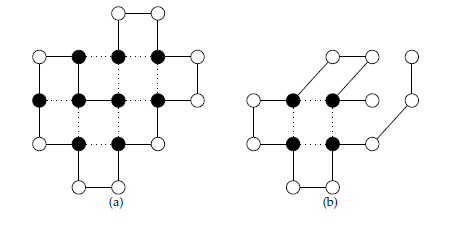
\includegraphics[scale=.9]{Imagens/modeloHPExemplo.png}
	\caption{Exemplos de representação de proteínas utilizando os modelos HP 2D-HP (a) e 3D-HP (b). Fonte: Adaptado de \cite{benitez2015algoritmo}}
	\label{fig:exemploModeloHP}
\end{figure}


Diversos trabalhos tem aplicado algoritmos de otimização ao problema de dobramento de proteínas utilizando o modelo HP. Uma decisão comum a todos trabalhos que utilizam o modelo HP é a de como representar as variáveis de entrada. Na literatura é possível encontrar basicamente três representações \cite{krasnogor1999protein, lopes2008evolutionary}: 

\begin{itemize}
	\item Coordenadas cartesianas: Este método  representa a posição de cada aminoácido utilizando suas coordenadas espaciais (x,y) no plano cartesiano 2D ou (x,y,z) no plano cartesiano 3D. Geralmente, sua utilização não é adequada para algoritmos baseados em população, pois estruturas idênticas ou semelhantes podem ter coordenadas totalmente diferentes  \cite{benitez2015algoritmo}; 
	\item Coordenadas internas: Nesta representação as conformações são representadas por conjuntos de movimentos que ditam como a estrutura final irá se parecer. Esta representação é a mais utilizada em abordagens com algoritmos evolucionários para o PDP \cite{benitez2015algoritmo}. Existem duas possibilidades de se representar conformações utilizando coordenadas internas:
	\begin{itemize}
		\item Coordenadas absolutas: Este tipo de coordenada é baseado na orientação do eixo da grade onde a conformação esta contida. No caso de uma grade bidimensional os possíveis movimentos são: $\{N,S,L,O\}$ ou norte,sul,leste e oeste. Já em uma grade 3D os possíveis movimentos são: $\{N,S,L,O,F,T\}$ que correspondem aos mesmos movimentos no caso 2D porém com dois movimentos a mais: para frente e para trás.
		\item Coordenadas relativas: Este tipo de representação define a posição de cada aminoácido da cadeia em relação ao movimento do seu predecessor. O conjunto de movimentos possíveis para a grade 2D é definido por $\{F,E,D\}$, que correspondem aos movimentos: frente (continuar no mesmo sentindo do aminoácido anterior), à esquerda e à direita. Em um cubo 3D, os possíveis movimentos são $\{F,E,D,C,B,\}$, possuindo dois movimentos a mais: para cima e para baixo. 
	\end{itemize}
	\item Matriz de distâncias: descreve a conformação de uma proteína através de uma matriz quadrada que representa a distância entre os aminoácidos. Este tipo de representação é raramente utilizado na literatura \cite{benitez2015algoritmo}.
\end{itemize}



\subsubsection{Outros Modelos}


Além do modelo HP, outros modelos simples em grade são utilizados para representar a estrutura de proteínas em outros estudos encontrados na literatura. Por exemplo:

\begin{itemize}
	\item Modelo PH (\textit{Perturbed Homopolymer}): Proposto por Shakhnovich et al. \cite{shakhnovich1993engineering}, as reações entre aminoácidos hidrofóbicos não são levadas em consideração, mas as interações entre aminoácidos do mesmo tipo são favorecidas, ou seja, H-H e P-P, desfavorecendo ligações H-P \cite{benitez2015algoritmo}.
	\item Modelo LPE (\textit{Lattice Polymer Embedding}): Modelo proposto por Unger e Moult \cite{unger1993finding}. A modelagem é feita a partir de uma sequência de aminoácidos, A = $a_1,...a_n$ atrelada a uma grade cúbica. Cada aminoácido possui um coeficiente de afinidade, definido para cada par $a_i,a_j (c(a_i,a_j))$. O objetivo da função de energia é minimizar o produto dos coeficientes pela distância entre os aminoácidos \cite{benitez2015algoritmo}.
	\item Modelo HP-TSSC (\textit{Hydrophobic-Polar Tangent Spheres Side Chain Model}): este modelo
	proposto por Hart et al. \cite{hart1997lattice} é baseado no modelo HP, porém não
	utiliza uma grade. Neste modelo a proteína é modelada via um grafo tridimensional, onde a cadeia lateral e o \textit{backbone}
	de cada aminoácido são esferas de mesmo raio \cite{benitez2015algoritmo}.
	\item Modelo CGE (\textit{Charged Graph Embedding}): Modelo descrito por Ngo et al. \cite{ngo1994protein}. Neste modelo, uma carga (\textit{charge}) é atribuída a cada
	resíduo. Entretanto, as conformações permitidas não são realistas \cite{benitez2015algoritmo}. 
	\item Modelo HPNX: modelo proposto por Bornberg-Bauer \cite{bornberg1997chain}. Divide
	os 20 aminoácidos em 3 classes: hidrofóbicos (H), positivos (P), negativos
	(N) e neutros (X). Este modelo, assim como o modelo HP, utiliza uma grade. Interações entre aminoácidos hidrofóbicos (H-H) representam
	interações de atração e diminuem a energia da conformação em 4,0,
	as interações entre positivos (P-P) e negativos (N-N) representam interações de repulsão e aumentam a energia livre em 1,0 e as interações entre N e P decrescem a energia em 1,0. O objetivo também consiste em minimizar a energia livre. Da mesma maneira que o modelo HP, quanto mais interações hidrofóbicas melhor será o dobramento. Porém este modelo não desconsidera o valor das demais interações \cite{benitez2015algoritmo}.
	\item Modelo HP-helicoidal (Helical-HP): este modelo proposto por Thomas e Dill \cite{thomas1993local} considera apenas uma grade bidimensional e inclui dois tipos de interação: interações não-locais através de energia de contatos hidrofóbicos e interações locais representadas por uma tendência à formação de a-hélices (chamada de propensão hélica) \cite{benitez2015algoritmo}.
	\item Modelo \textit{off-lattice} AB: este modelo proposto por Stillinger et al. \cite{stillinger1993toy} divide os aminoácidos em duas classes de acordo com sua polaridade: Hidrofóbicos (A) e Hidrofílicos (ou polares  B). Inicialmente, este modelo foi aplicado em duas dimensões (2D AB \textit{off-lattice}) e posteriormente aplicado para três dimensões (3D AB \textit{off-lattice}). Os aminoácidos não consecutivos interagem através de um potencial modificado de Lennard-Jones. Os ângulos de torsão entre ligações sucessivas também contribuem no cálculo da função de energia \cite{benitez2015algoritmo}.
	
\end{itemize}




\subsection{Considerações Finais}
\label{Problema de Dobramento de Proteínas:Conclusao}

Nesta Capítulo foi apresentado o problema de dobramento de proteinas, bem como sua importância para biológica computacional, química orgânica e medicina. Também foi mencionado que existem diversos modelos para representar estruturas de proteínas. Cada modelo tem suas peculiaridades e considera interações diferentes. Não existe um modelo que represente de maneira real o dobramento de proteínas, pois se trata de um processo ainda não completamente compreendido pelos cientistas e pesquisadores. Os modelos propostos tem diferentes níveis de detalhe e complexidade. O modelo mais simples é o HP mas apesar da sua simplicidade se apresenta como um problema $NP$-completo. O modelo HP é utilizado nesta proposta por conta de sua simplicidade de implementação, assim como o baixo custo computacional para realizar simulações do cálculo de energia. Existem diversas maneiras de representar as soluções utilizando o modelo HP. Nesta dissertação será utilizada a representação relativa pois, é mencionado na literatura que esta tem uma maior capacidade de guiar algoritmos de busca a melhores resultados  \cite{krasnogor1999protein}.

\chapter{Referencial Teórico}
\label{cap:Referencial Teórico}

% figuras estão no subdiretório "figuras/" dentro deste capítulo
\graphicspath{\currfiledir/figuras/}


\section{AEs - Algoritmos Evolucionários}

Um algoritmo evolucionário (AE) é uma técnica de busca, altamente paralela, inspirada na teoria da seleção natural e reprodução genética de Charles Darwin. De acordo com a teoria de Darwin, a seleção natural irá favorecer os indíviduos que forem mais aptos, dessa maneira, estes indíviduos tem uma maior probabilidade
de reprodução. Indivíduos com mais descendentes tem uma chance maior de perpetuarem seus códigos genéticos nas gerações futuras. O código genético é a identidade de cada indivíduo e é representado por cromossomos. Estes princípios são utilizados na implementação de algoritmos computacionais, que procuram por soluções melhores para um dado problema, evoluindo uma população 
de soluções codificadas em cromossomos artificais -- estruturas de dados utilizadas para representar soluções factíveis para um dado problema \cite{pacheco1999algoritmos}.

De maneira geral, problemas reais de otimização possuem múltiplos objetivos a serem minimizados/maximizados e estão presentes em muitas áreas do conhecimento.
Para otimizar problemas multiobjetivos, dois ou mais objetivos são considerados os quais geralmenta são conflitantes. Para estes problemas é impossível encontrar uma
única solução ótima. Um conjunto de soluções é encontrado avaliando a dominância de Pareto \cite{pareto} entre as soluções. O objetivo principal é encontrar o conjunto  
de soluções que sejam não dominadas entre si. Uma solução domina outra, se e somente se, for melhor em pelos um dos objetivos, sem ser pior em qualquer outro.
Este conjunto de soluções constitui a fronteira de Pareto. Encontrar a fronteira real de Pareto é um problema NP-Completo \cite{fonseca2005tutorial}, dessa maneira,
o objetivo é encontrar uma boa aproximação da fronteira real.

Algoritmos Evolucionários Multi-Objetivos (AEMOs) são extensões de AEs para problemas multi-objetivos os quais aplicam
conceitos da dominância de Pareto para criar diferentes estratégias para evoluir e manter a diversidade das soluções.
Nesta dissertação foram explorados dois AEMOs: NSGAII \cite{deb2002fast} and IBEA \cite{zitzler2004indicator}.
%=====================================================

\subsection{NSGAII - Non-dominated sorting Genetic Algorithm II}

O algoritmo \ref{alg:nsgaII} apresenta o pseudo código do NSGAII. O algoritmo recebe como parâmetro $N$ o tamanho da população e $T$ o número máximo 
de avaliações. O algoritmo inicia criando uma população com tamanho $N$ chamada $P_0$. A população $P_0$ é classificada de acordo com aptidão 
e a relação de não dominância. A população $P_0$ é submitida ao operador de seleção: torneio binário para selecionar duas soluções que serão utilizadas
para gerar descendentes. Operadores de cruzamento e mutação são aplicados na soluções selecionadas gerando duas soluções distintas descendentes. 
Ao fim do processo de reprodução as soluções descendentes são avaliadas e adicionadas a população chamada $Q_0$.

Após esta estapa, $P_0$ e $Q_0$ são adicionadas em uma população auxiliar chamada $R$. Utilizando o conceito de não dominância, $R$ é ordenada 
criando fronteiras, onde cada solução da primeira fronteira não é dominada por nenhuma outra solução, já soluções da segunda fronteira são dominadas
apenas por soluções contidas na primeira fronteira, e assim por diante. Para cada fronteira, as soluções são avaliadas utilizando um mecanismo
de \textit{Crowding-Distance} as soluções com maiores valores irão ser adicionadas na população da próxima geração chamada $P_t$ onde $t$ é a
avaliação corrente.

Após criar e preencher $P_t$ com as soluções não dominadas de todas as fronteiras, a população $P_t$ é avaliada e então passa para um novo
torneio binário e reprodução, dessa maneira, iniciando uma novo ciclo do algoritmo.

\begin{algorithm}[htb!]
	\begin{algorithmic}[1]
		\State{$N \gets$ Population Size}
		\State{$T \gets$ Max evaluations}
		\State{$P_0 \gets CreatePopulation(N);$}
		\State{$CalculateFitness(P_0);$}
		\State{$FastNonDominatedSort(P_0);$}
		\State{$Q_0 \gets 0$}
		\While{$Q_0 < N$}
		\State{$Parents \gets BinaryTournament(P_0);$}
		\State{$Offspring \gets CrossoverMutation(Parents);$}
		\State{$Q_0 \gets Offspring$}
		\EndWhile
		\State{$CalculateFitness(Q_0);$}
		\State{$t \gets 0$}
		\While{$t < T$}
		\State{$R_t \gets P_t \cup Q_t;$}
		\State{$Fronts \gets FastNonDominatedSort(R_t);$}
		\State{$P_{t+1} \gets 0$}
		\State{$i \gets 0$}
		\While{$P_{t+1} + Front_i  < N$}
		\State{$CrowdingDistanceAssignment(Front_i);$}
		\State{$P_{t+1} \gets P_{t+1} \cup Front_i$}
		\State{$i \gets i + 1$}
		\EndWhile
		\State{$CrowdingDistanceSort(Front_i);$}
		\State{$P_{t+1} \gets P_{t+1} \cup Front_i[1:(N -P_{t+1})]$}
		
		\State{$Parents \gets BinaryTournament(P_{t+1});$}
		\State{$Q_{t+1} \gets CrossoverMutation(Parents);$}
		\State{$t \gets t +1$}
		\EndWhile
		\State{\Return{$P \gets$ Set of non-dominated solutions.}}
	\end{algorithmic}
	\caption{NSGAII}
	\label{alg:nsgaII}
\end{algorithm}


%=====================================================

\subsection{IBEA (Indicator-Based Evolutionary Algorithm)}

No contexto de otimização multiobjetiva, otimizar consiste em tentar encontrar a fronteira com uma boa aproximação da fronteira real de Pareto. 
Entretanto, não existe uma definição geral para "uma boa aproximação". Consequentemente, indicadores de qualidade vem sendo utilizados
para avaliar a qualidade da aproximação de fronteiras. O indicador \textit{hypervolume} é um exemplo de indicador utilizado para avaliação e comparação 
das fronteiras.

No algoritmo IBEA, indicadores de qualidade são	utilizados para avaliar o conjunto de soluções não dominadas \cite{figueiredo2013algoritmo}.
Para utilizar o IBEA, é necessário definir qual indicador será utilizado para associar cada solução a um valor scalar. Um dos indicadores bastante utilizados
em conjunto com IBEA é o \textit{hypervolume} por conta da sua capacidade de avaliar a convergência e a diversidade do espaço de busca ao mesmo \cite{ishibuchi2008evolutionary}.

\begin{equation} \label{eq:ibeaFitness}
F(x_i) = \sum_{x_j \in (P-x_i)} {-e^\frac{-I_{Hy}(x_j,x_i)}{k}}
\end{equation}

A equação de \textit{fitness} do IBEA é apresentada pela equação \ref{eq:ibeaFitness} e é utilizada para calcular a contribuição de uma dada solução
para o valor do indicador referente a população, onde $k$ é um fator escalar dependente do $I_{Hy}$, o qual representa o indicador de qualidade sendo utilizado.
O valor $F(x_i)$ corresponde à perda de qualidade da aproximação, da fronteira real de Pareto, se a solução $x_i$ for removida da população \cite{figueiredo2013algoritmo}.


O Algoritmo \ref{alg:ibea} recebe como parametro o tamanho da população $N$, o número máximo de avaliações $T$ e o fator escalar $k$. O processo se inicia
criando uma população $P$ de tamanho $N$. Até que o critério de parada seja atingido os seguintes passos irão se repetir: um torneio binário 
para selecionar indivíduos, reprodução (cruzamento e mutação) dos indivíduos selecionados para gerar descendentes, adicionar os descedentes na população
auxiliar $\overline P$. Após a reprodução, a população $\overline P$ é unida com $P$. Enquanto o tamanho de $P$ exceder $N$, o pior indíviduo avaliado
pela equação \ref{eq:ibeaFitness} é removido da população $P$ e os indíviduos restantes são re-avaliados. Quando o algoritmo terminar irá retornar o conjunto
de soluções não dominadas é retornado.

\begin{algorithm}[htb!]
	\begin{algorithmic}[1]
		\State{$N \gets$ Population Size}
		\State{$\overline N \gets$ AuxiliaryPopulationSize}
		\State{$T \gets$ Max Evaluations}
		\State{$k \gets$ Scale factor of Fitness}
		
		\State{$P \gets$ CreatePopulation($N$);}
		\State{$\overline P \gets$ CreateEmptyAuxiliaryPopulation($\overline N$);}
		\State{$m \gets 0$}
		\State{CalculateFitness($P$);}
		
		\While{$m \ge T$ or other stop criterion is not reached}
		
		\State{$\overline P \gets$ BinaryTournament($P$);}
		\State{$\overline P \gets$ CrossoverMutation($\overline P$);}
		\State{$P \gets P \cup \overline P$}
		\State{$m \gets m+1$}
		
		\While{Size($P$) $> N$}
		\State{$x^* \gets$ WorstIndividualByFitness();}
		\State{RemoveFromPopulation($x^*$, $P$);}
		\State{CalculateFitness($P$);}
		\EndWhile
		
		\EndWhile
		\State{\Return{$P \gets$ Set of non-dominated solutions}}
		
	\end{algorithmic}
	\caption{IBEA}
	\label{alg:ibea}
\end{algorithm}

%\footnotetext[1]{\textit{Hypervolume}: Indicador de qualidade utilizado neste estudo \cite{zitzler1998multiobjective}, 
%	denotado como o "tamanho da área coberta do espaço de busca". Este indicador tem uma vantagen importante em relação aos outros \cite{zitzler2007hypervolume}:
%	1 - Sensitivo a qualquer tipo de melhoria na aproximação em relação a outro conjunto. 

\section{Hiper-Heurísticas }
\label{Hiper-Heuristicas}

Apesar do sucesso de métodos heurísticos e outros métodos de busca na tarefa de resolver problemas de busca computacional difíceis ainda existem dificuldades em generalizar estes métodos para diferentes problemas ou até mesmo para diferentes instâncias de um mesmo problema. Esta dificuldade provém principalmente da necessidade de selecionar os parâmetros e configurações mais adequados dos algoritmos para um problema ou para uma dada instância de um problema. Também vale mencionar a pouca orientação na tarefa de definir estes parâmetros.  É neste contexto que surge uma questão: é possível automatizar o projeto e parametrização de métodos heurísticos para resolver problemas de busca computacional difíceis? \cite{burke2013hyper}. A ideia principal é desenvolver algoritmos que sejam mais genéricos do que as implementações de metodologias atuais \cite{burke2013hyper}. As principais abordagens já propostas para este desafio podem ser classificadas em duas categorias: configuração estática (\textit{offline}) e controle dinâmico (\textit{online}). Abaixo são apresentadas algumas abordagens já propostas na literatura:

\begin{itemize}
	\item Configuração Estática (Offline):
	\begin{itemize}
		\item Seleção de algoritmos;
		\item Portfólio de algoritmos;	
		\item Configuração de algoritmos;
		\item Ajuste de parâmetros;
		\item Hiper-Heurísticas.
	\end{itemize}
	\item Controle Dinâmico (Online):
	\begin{itemize}
		\item Seleção adaptativa de operadores (AOS);
		\item Controle de parâmetros;	
		\item Algoritmos meméticos adaptativos;
		\item Hiper-Heurísticas
	\end{itemize}
	
\end{itemize}


Esta seção tratará apenas de hiper-heurísticas e suas particularidades. Uma hiper-heurística pode ser vista como uma metodologia de alto nível, a qual seleciona ou cria heurísticas para resolver um dado problema ou instância de um problema. \cite{burke2013hyper}. O objetivo principal é tentar encontrar ou construir a heurística mais adequada para cada situação. As hiper-heurísticas diferem dos métodos padrão de busca pois operam sobre o espaço de busca de heurísticas que por sua vez operam sobre o espaço de busca de um problema. Além disso, hiper-heurísticas são independentes do problema. Tradicionalmente frameworks hiper-heurísticos possuem dois níveis: \cite{sabar2014automatic}

\textbf{Heurísticas de baixo nível}:  Um conjunto de heurísticas de baixo nível específicas. Estas heurísticas costumam diferir entre domínios de problemas. São exemplos: operadores de cruzamento, mutação e buscas locais. Em alguns casos, meta-heurísticas também, dependendo da modelagem do \textit{framework} hiper-heurístico, podem assumir o papel de heurísticas de baixo nível. 

\textbf{Heurísticas de alto nível}: Geralmente consistem em dois componentes: mecanismo de seleção, que gerencia quais heurísticas de baixo nível devem ser aplicadas durante a busca; um critério de aceitação, que tem a responsabilidade de decidir se irá aceitar ou não uma solução gerada, a partir da aplicação de uma heurística de baixo nível. A responsabilidade do mecanismo de seleção é selecionar, de um \textit{pool} de heurísticas de baixo nível, a heurística que for mais adequada naquele momento. Geralmente, a escolha da heurística de baixo nível é crucial para uma boa exploração do espaço de busca, evitando que a busca fique confinada em uma região específica \cite{sabar2015automatic}. O objetivo do critério de aceitação é auxiliar o processo de busca a evitar mínimos locais assim como explorar diferentes regiões através do aceite ou rejeição de soluções geradas \cite{chakhlevitch2008hyperheuristics}. Espera-se que um bom critério de aceitação deva atingir um bom equilíbrio entre aceitar soluções melhores assim como soluções diversificadas se a busca estiver presa em um mínimo local \cite{sabar2015automatic}. Ambos os componentes devem ser independentes de conhecimento sobre o problema.

A imagem \ref{img:hiperheuristico} apresenta um diagrama exemplificando os níveis de um \textit{framework} hiper-heurístico e suas características. Note que entre os níveis (alto e baixo) existe uma barreira de domínio, ou seja, apenas as heurísticas de baixo nível são dependentes de conhecimento do problema ou instância e as heurísticas de alto nível não são dependentes do problema. 

\begin{figure}[!htb]
	\centering
	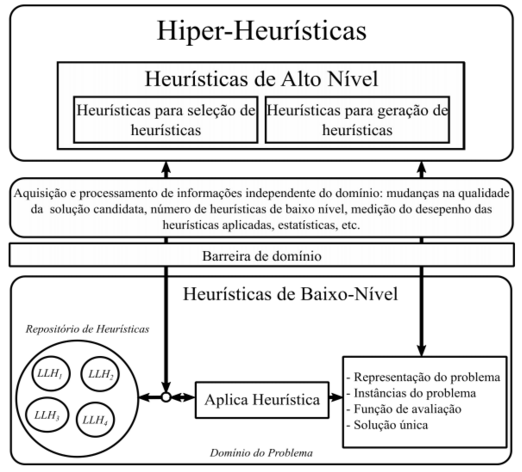
\includegraphics{Imagens/HiperHeuristicas.png}
	\caption{Framework Geral Hiper-Heurístico. Adaptado de \cite{sabar2015automatic}}
	\label{img:hiperheuristico}
\end{figure}


Como cada instância ou problema possui um espaço de busca com diferentes características, os componentes da heurística de alto nível têm um grande impacto no desempenho de um \textit{framework} hiper-heurístico. Esta é uma das razões de existir um grande interesse de pesquisa em desenvolver  novos mecanismos de seleção, assim como diferentes critérios de aceitação \cite{burke2013hyper}. Um bom mecanismo de seleção deve selecionar a heurística mais adequada em um dado momento, para guiar a busca para regiões promissoras do espaço de busca. 
Ao utilizar hiper-heurísticas, espera-se encontrar o método correto ou a sequência de heurísticas que mais se adequam a um problema ou instância ao invés de tentar resolver o problema diretamente. Entretanto, um importante objetivo é desenvolver métodos genéricos, que têm  potencial em produzir soluções com uma qualidade aceitável, utilizando um conjunto de heurísticas de baixo nível fácil de implementar. As hiper-heurísticas podem ser classificadas de diversas maneiras. A figura \ref{img:classificacaoHiperHeuristicas} apresenta as possíveis classificações descritas na literatura. 

\begin{figure}[!htb]
	\centering
	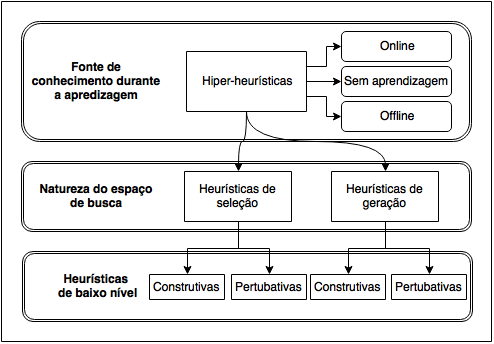
\includegraphics[scale=0.8]{Imagens/ClassificacaoHiperHeuristica.png}
	\caption{Classificação Hiper-heurísticas. Adaptado de \cite{sabar2015automatic}}
	\label{img:classificacaoHiperHeuristicas}
\end{figure}

A primeira classificação de hiper-heurísticas é baseada na sua fonte de conhecimento durante a busca: \textit{Online} é quando a hiper-heurística toma decisões de maneira instantânea, baseando-se em métricas durante sua execução, não necessitando de treinamento prévio. \textit{Offline} necessita de treinamento prévio; estes \textit{frameworks}  tomam suas decisões baseados no que foi aprendido apenas durante o treinamento, sem atualização deste conhecimento. Os \textit{frameworks} classificados como \textit{No-Learning} não possuem nenhuma forma de aprendizagem. Outra classificação considera como as heurísticas de baixo nível operam sobre as soluções do problema. As heurísticas ditas perturbativas realizam pequenas perturbações nas soluções gerando novas soluções. Já heurísticas construtivas criam soluções do zero passo a passo e normalmente avaliam cada etapa da construção para obter \textit{feedback} sobre o seu desempenho. Uma última  classificação, mas não menos importante, divide as hiper-heurísticas de acordo com a  natureza do seu espaço de busca. As hiper-heurísticas de seleção selecionam sequências de heurísticas a serem aplicadas para resolver um dado problema ou instância. Já as hiper-heurísticas de geração operam gerando novas heurísticas com objetivo de resolver um problema ou instância.


\subsection{Hiper-heurísticas de Geração}
\label{Hiper-Heuristicas-Geraçao}

Estas hiper-Heurísticas geram novas heurísticas combinando componentes de heurísticas existentes. Geralmente se utiliza programação genética (GP), ou alguma vertente de GP, como por exemplo evolução gramatical \cite{ryan1998grammatical} ou programação gênica \cite{ferreira2006gene}, como hiper-heurística para gerar heurísticas. A próxima sub-seção irá introduzir o conhecimento necessário para a compreensão da programação genética, assim como irá introduzir evolução gramatical, que se trata de um tipo de programação genética e que será utilizada nesta proposta.

\section{Programação Genética (PG)}
\label{subsection:PG}

Programação Genética \cite{burke2009exploring} é um ramo da síntese de programas que utiliza ideias oriundas da teoria da evolução natural para produzir programas. Os principais componentes da computação evolucionária são herança (cruzamento/reprodução), seleção e variação (mutação). A herança significa que os descendentes  têm alguma semelhança com seus pais, pois quase todo material genético vem dos pais. A seleção trata de escolher quais pais irão se reproduzir para gerar novos descendentes; pais com maior aptidão tendem a ter maior probabilidade de serem selecionados. Esta pressão de seleção define quais indivíduos estão mais aptos que outros. Variação realiza pequenas alterações em um descendente a fim de criar novo material genético neste indivíduo e que não estava presente em nenhum dos indivíduos que o geraram. Computação evolutiva pode ser pensada como a interação destes três componentes. 
Uma população aleatória de programas de computador é gerada, e os operadores geneticamente inspirados (cruzamento e mutação) são repetidamente aplicados com objetivo de produzir novos programas de computador. Estes programas são avaliados utilizando uma função de \textit{fitness} (normalmente dependente do desempenho obtido pela aplicação do programa em um problema), que determina quais destes programas são mais suscetíveis a sobreviver para gerações futuras. Os programas com maior aptidão tem mais chances de serem selecionados para o cruzamento e perpetuarem parte de seus códigos genéticos durante o processo evolutivo. 
Programação genética é um método de geração de programas sintaticamente válidos e a função de \textit{fitness} é utilizada para decidir quais programas são mais adequados para o problema.
Na programação genética, os programas que compõem a população são tradicionalmente representados utilizando estruturas de árvore. Existem outras estruturas que podem ser evoluídas, como por exemplo: sequências lineares de instruções ou gramáticas. Nesta proposta será utilizada uma representação gramatical linear que será explicada na seção \ref{subsubsection:EvolucaoGramatical}.

\section{Evolução Gramatical (EG)}
\label{subsubsection:EvolucaoGramatical}

Evolução gramatical é uma técnica relativamente nova de computação evolutiva, proposta por Ryan et al. \cite{ryan1998grammatical}, trata-se de um tipo de programação genética. Assim como na programação genética, o principal objetivo é encontrar um programa executável ou trecho de um programa, que obtenha um bom valor de \textit{fitness} para o problema em questão. Na maioria dos trabalhos publicados de programação genética, expressões que representam estruturas de árvore são manipuladas, enquanto na evolução gramatical os operadores genéticos são aplicados em vetores de inteiros que posteriormente são mapeados para um programa (ou trecho de programa) através de uma gramática específica. Um dos benefícios de EG é que este mapeamento generaliza a aplicação para diferentes linguagens de programação.
Ryan el al. \cite{ryan1998grammatical} propõem uma técnica para gerar programas ou fragmentos de programas para qualquer linguagem de programação utilizando definições BNF. A técnica pode ser utilizada para evoluir programas por um processo evolutivo. A evolução gramatical adota um mecanismo de mapeamento entre o genótipo (indivíduos codificados em um vetor de inteiros) e o fenótipo (programas gerados para resolver algum problema). 
A notação \textit{Backus Naur Form} (BNF) é a notação utilizada para expressar a gramática de uma linguagem na forma de regras de produção. Uma gramática BNF consiste em um conjunto de terminais, os quais são itens que podem aparecer na linguagem, por exemplo: +, -, *, / etc e não terminais, que podem ser expandidos em um ou mais terminais e não terminais. Uma gramática pode ser expressada como uma tupla ${N,T,P,S}$, onde $N$ é o conjunto de não terminais, $T$ o conjunto de terminais, P um conjunto de regras de produção que mapeia os elementos $N$ para $T$; e, por último, $S$, um símbolo de início e que está contido em $N$.

\begin{center}
	
	$ N = {\langle expr \rangle, \langle op \rangle, \langle pre-op \rangle}$
	
	$ T = {Sin,Cos,Tan,Log,+,-,/,*,X} $
	
	$ S = \langle expr \rangle $
	
\end{center}

\noindent
E $P$ pode ser representada como:

\begin{Grammar}
	\begin{grammar}
		
		
		<expr> ::=  <expr> <op> <expr> \hspace{10cm} (0) 
		\alt (<expr> <op> <expr>) \hspace{9.7cm} (1)  
		\alt <pre-op> (<expr>) \hspace{10.15cm} (2) \alt <var> \hspace{12.1cm} (3) \\\
		
		<op> ::=  + \hspace{12.7cm} (0)   \alt - \hspace{12.8cm} (1)  \alt  /  \hspace{12.85cm} (2) \alt * \hspace{12.75cm} (3) \\
		
		<pre-op> ::= Sin  \hspace{12.4cm} (0) \alt Cos
		\hspace{12.3cm} (1) \alt Tan  \hspace{12.35cm} (2)
		
		<var> ::= X  \hspace{12.6cm} (0)
		
		
	\end{grammar}
	
	\caption{Gramática exemplo para demonstrar como decodificar vetores de inteiros em programas de computador.}
	\label{gram:gramatica}
\end{Grammar}


\begin{table}[htb]
	\centering
	\caption{\textit{Regras de produção} e o número de escolhas para cada uma.}
	\label{tab:productionRules}
	\begin{tabular}{|l|l|}
		\hline
		Regra de produção & Número de escolhas \\ \hline
		$\langle expr \rangle$                        & 4       \\ \hline
		$\langle op \rangle$                         & 4       \\ \hline
		$\langle pre-op \rangle$                         & 3       \\ \hline
		$\langle var \rangle$                          & 1       \\ \hline
	\end{tabular}
\end{table}


Ryan et al. \cite{ryan1998grammatical}  propôs o uso de um algoritmo genético (AG) para controlar quais escolhas devem ser feitas, permitindo dessa maneira que o AG controle quais regras de produção serão utilizadas. Um indivíduo (cromossomo) consiste em um vetor de tamanho variável de valores inteiros que representa o genótipo. Para fins de compreensão o processo de mapeamento de um cromossomo será demonstrado utilizando a \autoref{gram:gramatica} apresentada anteriormente nesta seção. O Algoritmo \ref{alg:pseudocodigogrammar} apresenta o \textit{template} geral dos programas gerados pela \autoref{gram:gramatica}. A expressão $\langle expr \rangle$ apresentada na linha 2 do Algoritmo \ref{alg:pseudocodigogrammar} é substituída por expressões matemáticas que estão codificadas pelos cromossomos (vetores de inteiros). 

\begin{algorithm}
	\caption{\textit{Template} geral dos algoritmos gerados}
	\label{alg:pseudocodigogrammar}
	float symb(float x) { \\
		a = $\langle expr \rangle$;   \\
		return a;  \\
	}	
\end{algorithm}

\noindent
Suponha o seguinte vetor de inteiros:

\begin{center}
	$ [220, 203, 17, 6, 108, 215, 104, 30] $
\end{center}


Este vetor será utilizado para mapear o cromossomo (genótipo) em um trecho de programa (fenótipo) utilizando a gramática BNF. 
%A expressão não terminal $ \langle expr \rangle$ no algoritmo \ref{alg:pseudocodigogrammar} será preenchida por um trecho de código que será mapeado a partir do cromossomo apresentado. Os passos do mapeamento serão descritos a seguir.%
A tabela \autoref{tab:productionRules} resume o número de escolhas associada à cada regra de produção da \autoref{gram:gramatica}. Existem 4 opções de regras de produção que podem ser selecionadas para a expressão $ \langle expr \rangle$. Para decidir qual será selecionada, o primeiro valor no cromossomo deve ser utilizado. O valor é 220. Devemos realizar o módulo deste valor pelo número de escolhas, neste caso 4. Portanto, 220 MOD 4 = 0, o que significa selecionar a primeira opção: $\langle expr \rangle \langle op \rangle \langle expr \rangle$.

Note que a primeira expressão é novamente $ \langle expr \rangle$ e da mesma maneira devemos obter o próximo valor de inteiro e realizar o módulo. O próximo valor inteiro é 203; realizando o modulo de 4, resulta em 3, que portanto seleciona a quarta opção: $ \langle var \rangle$. Substituindo na expressão anterior, obtemos: $ \langle var \rangle \langle op \rangle \langle expr \rangle$

Nenhuma escolha é necessária para a expressão $ \langle var \rangle$, pois existe apenas uma opção $X$. A expressão pode ser reescrita da seguinte maneira: $X \langle op \rangle \langle expr \rangle$

Neste momento é necessário decodificar a expressão não terminal $\langle op \rangle$. Obtendo o próximo valor inteiro do cromossomo, temos 17 e para o $ \langle op \rangle$ temos 4 opções $(+ | - | / | *)$. O resultado de 17 MOD 4  é igual a 1, que significa selecionar:  $-$. Substituindo na expressão, temos: $X  -  \langle expr \rangle$


Novamente é necessário fazer uma nova escolha para resolver a expressão não terminal $\langle expr \rangle$. O próximo valor do cromossomo é 6 e novamente existem 4 opções. Realizando o modulo 6 MOD 4, obtém-se 2, que seleciona $ \langle pre-op \rangle ( \langle expr \rangle)$. Atualizando a expressão, obtemos: $X - \langle pre-op \rangle (\langle expr \rangle)$

Resolvendo a expressão $ \langle pre-op \rangle$, obtemos 108 MOD 4 = 0 que por sua vez seleciona a primeira expressão  terminal $Sin$. Atualizando a expressão, obtemos: $X - Sin (\langle expr \rangle)$

Expandindo $ \langle expr \rangle$, obtemos 215 MOD 4 = 3, que seleciona a expressão não terminal $ \langle var \rangle$. Já que para a expressão $ \langle var \rangle$ existe apenas uma opção, nenhuma escolha é necessária e a expressão final decodificada (fenótipo) é: $X - Sin (X)$

Note que nem todos os genes do cromossomo foram necessários para obter o fenótipo. Nos casos em que isto ocorre, os genes que não forem utilizados são desconsiderados. Além disso, pode ocorrer que um cromossomo não tenha genes suficientes para mapear um programa. Neste caso a estratégia é reutilizar os genes do cromossomo a partir do primeiro gene. 

Operadores genéticos tradicionais (cruzamento e mutação) também são utilizados na EG. Além dos operadores tradicionais outros dois operadores \textit{Prune} e \textit{Duplicate} são peculiares à EG e serão descritos em seguida:

\begin{itemize}
	\item \textit{Duplicate}: Este operador (dada uma probabilidade) realiza a cópia de  alguns genes. Os genes duplicados são adicionados após a última posição do cromossomo. O número de genes a serem duplicados é selecionado de maneira aleatória. A motivação por trás deste operador é que ao duplicar genes ocorre um aumento da presença de genes que são potencialmente bons, pois pertencem a um indivíduo com boa aptidão selecionado pelo operador de seleção.
	\item \textit{Prune} : Este operador leva em consideração que nem sempre todos os genes, de um cromossomo, são utilizados para decodificar um programa. Dessa maneira (dada uma probabilidade) realiza o truncamento de  cromossomos. O objetivo é diminuir a probabilidade que o operador de cruzamento opere em regiões dos cromossomos que não sejam utilizadas realmente.
\end{itemize}


O Algoritmo \ref{alg:GE} apresenta o pseudocódigo da evolução gramatical (EG). Note que o pseudocódigo é muito similar a um algoritmo genético simples. Nas linhas 3 e 4 ocorre a inicialização da população e o mapeamento para programas utilizando a gramática que foi provida como entrada. Em seguida, na linha 5 ocorre a execução dos programas e na linha 6 acontece a avaliação dos indivíduos da população, baseando-se na saída obtida pelos respectivos programas. Dentro do laço principal, apresentado na linha 7, podemos observar o processo de seleção dos indivíduos pais na linha 8 e na linha 9 o processo de cruzamento destes indivíduos. Nas linhas 10 e 11 ocorre a aplicação dos operadores \textit{Prune} e \textit{Duplicate} respectivamente e na linha 12 podemos observar a aplicação do operador de mutação. Em seguida, nas linhas 13,14 e 15 ocorre o mapeamento dos indivíduos descendentes para programas, execução dos programas e finalmente a atribuição de \textit{fitness} para os descendentes. Por fim, na linha 16 do laço principal, ocorre a substituição dos descendentes na população. 


%exceto pela aplicação dos operadores \textit{Duplicate} e \textit{Prune} (linhas 10 e 11 do Algoritmo  \ref{alg:GE}) e o processo de decodificação e execução dos programas descendentes (linhas 13 e 14 do Algoritmo \ref{alg:GE}).

\begin{algorithm}[htb!]
	%\fontsize{8pt}{10pt}\selectfont
	
	
	\begin{algorithmic}[1]
		\State{$AG  \gets$ Arquivo da gramática;}
		\State{$populacao \gets$ Inicialização a população;}
		\State{$programas \gets$ Mapeia $populacao$ para programas utilizando $AG$;}
		\State {Executa os $programas$;}
		\State {Atribui valor de \textit{fitness} para as soluções  of $populacao$ de acordo com a saída obtida pelos respectivos programas decodificados;}
%		\While{Condição de parada não atingida}
		\While{Condição de parada não atingida}
			\State {$pais \gets $ Seleção de indivíduos para cruzamento;}
			\State {$descendentes \gets$ Cruzamento $pais$;}
			\State {Aplica o operator \text{Prune} nas soluções $descendentes$;}
			\State {Aplica o operador \textit{Duplicate} nas soluções $descendentes$;}
			\State {Aplica o operador de mutação nas soluções $descendentes$;}
			\State {$programas \gets$ Mapeia $descendentes$ para programas utilizando $AG$;}
			\State {Executa $programas$;}
			\State {Atribui valor \textit{fitness} para as soluções $descendentes$ de acordo com a saída obtida pelos respectivos programas decodificados;}
			\State 	{$populacao \gets$ Realiza substituição;}
		\EndWhile \\
		\Return{Melhor programa da $populacao$;}
			
			
		
	\end{algorithmic}
	\caption{Pseudocódigo da evolução gramatical}
	\label{alg:GE}
\end{algorithm}


\section{Programação Genética como Hiper-Heurística de Geração de Heurísticas}
\label{subsubsection:PGasHH}

Nesta seção serão apresentadas questões relativas ao uso de EG como mecanismo de geração de heurísticas. 
Burke et al. \cite{burke2009exploring} descrevem que muitos autores mencionam a melhor adequação de programação genética, em relação a outras técnicas de aprendizagem de máquina, para gerar heurísticas de maneira automática. Burke et al \cite{burke2009exploring} também apontam algumas vantagens desta técnica:

\begin{itemize}
	\item PG utiliza cromossomos de tamanho variável. Geralmente, não se sabe um tamanho ótimo para representar heurísticas de um dado domínio de problema.
	\item PG produz estruturas de dados executáveis. E heurísticas são tipicamente expressadas como programas ou algoritmos.
	\item Facilidade em identificar boas características do domínio do problema, afim de definir o conjunto terminal que será utilizado pela PG.
	\item Heurísticas desenvolvidas por humanos podem facilmente ser expressadas na mesma linguagem utilizada para criar o espaço de busca da PG. O conjunto de funções, relevante para o problema pode ser determinado facilmente. E adicionalmente PG pode ser suplementada com uma gramática específica.
\end{itemize}

Todas estas vantagens descritas por Burke et al. \cite{burke2009exploring} também são consideradas ao utilizar EG, visto que se trata de uma extensão de programação genética e possui as mesmas características (cromossomo de tamanho variável, produz estruturas executáveis, etc).
Burke et al. \cite{burke2009exploring} também mencionam desvantagens, por exemplo: a cada execução da programação genética é encontrada uma melhor heurística que, por se tratar de uma técnica estocástica, os resultados podem ser distintos em diferentes execuções. Portanto se fazem necessárias múltiplas execuções, a fim de se obter um melhor conhecimento da qualidade das heurísticas que podem ser produzidas. Outra desvantagem é referente à configuração de parâmetros, que normalmente é encontrada via tentativa e erro.

\subsubsection{Abordagem Básica}

Burke et al. \cite{burke2009exploring} descrevem uma abordagem básica para aplicar programação genética para gerar heurísticas:

\begin{enumerate}
	\item Examinar as heurísticas existentes: Avaliar se as heurísticas já propostas para um dado problema podem ser descritas em um \textit{framework} comum. Estas heurísticas podem ter sido criadas por humanos ou até mesmo concebidas via outras técnicas de aprendizagem. Este passo não é trivial, pois envolve o entendimento de um número diverso de heurísticas existentes, que podem operar de diferentes maneiras. Geralmente heurísticas desenvolvidas por humanos são produtos de anos de pesquisa, portanto uma boa compreensão das heurísticas existentes pode ser um trabalho difícil. 
	\item Um framework que utilizará as heurísticas: neste momento a preocupação é em como as heurísticas serão aplicadas para um dado problema. Em geral, os frameworks tendem a ser bem diferentes dependendo do domínio do problema. 
	\item Definição do conjunto terminal: neste passo a preocupação refere-se a variáveis que expressem o estado do problema. Estas variáveis irão compor os terminais da programação genética/evolução gramatical. Outros terminais também podem ser utilizados. Particularmente, constantes aleatórias podem ser úteis.
	\item Definição do conjunto de funções: é necessário definir como as variáveis estarão relacionadas ou combinadas entre si. Estes relacionamentos irão compor o conjunto de funções da programação genética/evolução gramatical. 
	\item Identificar uma função de \textit{fitness}: uma função de \textit{fitness} precisa ser identificada para o problema. Geralmente, uma função simples de aptidão não irá avaliar bem os cromossomos. Introduzir alguns parâmetros pode ajudar a encontrar uma mais adequada.
	\item Executar o framework: geralmente ao executar pela primeira vez um framework hiper-heurístico com programação genética, não serão produzidos bons resultados, devido à escolha dos parâmetros. Isto é observado especialmente em casos que o pesquisador é iniciante. Portanto é essencial que as definições de parâmetros sejam cuidadosamente investigadas.
\end{enumerate}




\section{Conclusão}
\label{ReferencialTeorico:Conclusão}

%TODO: mencionar os AEMOs aqui
Neste capítulo foram apresentados os conceitos que permeiam a área de estudo sobre hiper-heurísticas, tendo sido discutidos os seus níveis (alto e baixo) e as classificações encontradas na literatura.  Foram discutidas algumas estratégias para hiper-heurísticas de seleção e geração. As hiper-heurísticas de geração foram mais detalhadas, pois esta proposta visa o projeto  automático de heurísticas de alto nível. Foram apresentados os conceitos de PG e sua extensão EG, por se tratarem de estratégias comumente utilizadas para o projeto de hiper-heurísticas de geração de heurísticas. Também foram discutidas algumas vantagens e desvantagens referentes ao uso de PG para geração de heurísticas, além de demonstrar que a EG possui as mesmas características da PG, pois se trata de uma extensão que utiliza uma gramática para gerar os programas. O funcionamento geral da EG foi demonstrado utilizando uma gramática exemplo e um vetor de inteiros e, por fim, o pseudocódigo da evolução gramatical foi apresentado. A Seção \ref{sec:ProblemaDobramentoProteínas} apresenta o Problema de Dobramento de Proteínas e a Seção \ref{sec:Metodologia} apresentará a proposta da aplicação de EG a este problema.





		% fundamentação teórica
\chapter{Trabalhos Relacionados}
\label{cap:Trabalhos Relacionados}

Este capítulo irá apresentar alguns trabalhados relacionados com a presente proposta. Serão apresentados trabalhos que buscam construir/adaptar estratégicas heurísticas para encontrar melhores soluções ao PDP utilizando o modelo HP. Também serão apresentados alguns trabalhos que utilizam técnicas de programação genética para gerar heurísticas para diferentes problemas.


%Também será apresentado um trabalho que trata do \textit{design} automático de heurísticas de alto nível para um \textit{framework}  hiper-heurístico aplicado a problemas de \textit{benchmark} disponibilizados pelo \textit{software} HyFlex \cite{ochoa2012hyflex}.

O estudo, desenvolvido por \cite{unger1993genetic}, foi percussores, ao aplicar um algoritmo genético ao PDP com o modelo HP, utilizando operadores de cruzamento e mutação aprimorados. Os resultados apresentados superam um número significativo de estratégias tradicionais anteriores que utilizam métodos Monte Carlo para explorar as conformações. 

Um algoritmo genético multi memético foi proposto por \cite{krasnogor2002multimeme}. Esta estratégia combina um algoritmo genético e buscas locais selecionando a busca local que mais se adequar com a instância (sequência) sendo otimizada. Mais tarde este trabalho foi aprimorado com um estrategia \text{fuzzy} para as buscas locais, dessa maneira produzindo melhores resultados para o PDP.

Em \cite{hsu2003growth}, os autores utilizam um algoritmo de crescimento de cadeia, chamado \textit{pruned-enriched Rosenbluth method} (PERM). Esta estratégia se baseia em iterativamente construir uma conformação adicionando os aminoácidos um a um. 

A otimização de colônia de formigas também foi aplicada para o PDP nos trabalhos \cite{shmygelska2002ant,shmygelska2003improved}. Estas abordagens utilizam formigas artificiais com objetivo de construir as conformações para o modelo HP. Uma busca local também foi introduzida com objetivo de melhorar e manter a qualidade das soluções. 

No trabalho de \cite{santanna2008} é proposto a aplicação de diferentes algoritmos de estimação de distribuição (AED) para o PDP. Os AEDs são capazes de aprender a explorar as regularidades do espaço de busca utilizando modelos de dependência probabilísticos. Os autores compararam os resultados com as abordagens descritas anteriormente neste capítulo e constataram que a sua abordagem conseguiu atingir os valores ótimos para várias sequências de aminoácidos.

O estudo desenvolvido por \cite{lin2011protein} utiliza um algoritmo genético híbrido combinando um operador de mutação baseado na otimização por exame de partículas. Os resultados apresentados por Lin et al. se mostraram superiores aos apresentados por outros estudos, da época, que utilizam algoritmos evolutivos. Este trabalho também utiliza operadores de buscas locais que serão utilizados como heurísticas de baixo nível na presente proposta. 


Custódio et al. \cite{custodio2014multiple} desenvolveram um metodologia que consistiu modificar um algoritmo genético para selecionar os operadores de cruzamento e mutação de maneira dinâmica. Além disso, utilizaram um mecanismo baseado em \textit{crowding}  para manter a diversidade durante o processo de busca. Este trabalho apresentou bons resultados em relação a outros estudos que exploram algoritmos evolutivos. Os operadores genéticos utilizados deste trabalho também serão implementados como heurísticas de baixo nível nesta proposta. 


Lourenço et al. \cite{lourencco2012evolving} desenvolveram uma estratégia hiper-heurística utilizando evolução gramatical para geração e \textit{tuning} automático de algoritmos evolutivos. Neste trabalho uma gramática foi desenvolvida e contém os principais componentes de algoritmos evolutivos. Os resultados apresentados por Lourenço et al. provaram a habilidade da abordagem para evoluir algoritmos evolutivos. Os resultados obtidos pelos algoritmos evolutivos gerados pela evolução gramatical são competitivos com outras abordagens padrão.


O trabalho desenvolvido \cite{sabar2015automatic} propõe uma estratégia, utilizando \text{Gene Expression Programming} (GEP), de geração de heurísticas de alto nível para um \textit {framework} hiper-heurístico aplicado a diversos problemas de \textit{benchmark} contidos no \text{framework} HyFlex \cite{ochoa2012hyflex}. Este trabalho se difere dos apresentados anteriormente pois foi aplicado a domínios de problemas diferentes do PDP. Este trabalho motivou a presente proposta pois os resultados apresentados se mostraram promissores. A aplicação de uma vertente de programação genética para geração de heurísticas tem uma maior capacidade de explorar espaços de busca complexos (com muitos mínimos locais) e com muitas restrições.


%TODO: Melhorar essa parte em conjunto com as consideracoes finais
A presente proposta visa aplicar evolução gramatical (EG), pois apesar de possuir as mesmas características da GEP ela torna mais amigável a manipulação dos indivíduos. Isto ocorre pelo fato de representá-los utilizando vetores de inteiros enquanto a GEP utiliza vetores de strings para representação. Dessa maneira, a EG facilita a manipulação dos indivíduos por operadores genéticos (cruzamento de mutação). A principal diferença entre esta proposta e os outros trabalhos relacionados \cite{santana2008protein,shmygelska2002ant,shmygelska2003improved,hsu2003growth, krasnogor2002multimeme,krasnogor2002multimeme,unger1993genetic} é que este irá trabalhar em um nível acima: gerando heurísticas de alto nível para um \textit{framework} hiper-heurístico que será aplicado ao PDP enquanto os outros trabalham aplicando meta-heurísticas diretamente ao PDP. 





\section{Conclusão}
\label{TrabalhosRelacionados:Conclusão}

%TODO: Melhorar essa parte
Neste capítulo foram discutidos alguns estudos que utilizam algoritmos de busca para explorar o espaço de busca do PDP utilizando o modelo HP. Também foram discutidos trabalhos que aplicam PG como hiper-heurística de geração de heurísticas. Foram mencionadas diferentes estratégias de busca para o PDP e algumas destas estrategias servem de base para alguns componentes que esta proposta possui. Os operadores genéticos utilizados \cite{custodio2014multiple} e \cite{lin2011protein} serviram de matéria prima para as heurísticas de baixo nível desta proposta. O trabalho desenvolvido por \cite{sabar2015automatic} será utilizado como base na implementação da presente proposta, pois obteve bons resultados dessa maneira, demonstrando a habilidade do \textit{framework} proposto generalizar bem entre diferentes domínios de problemas.		% revisão bibliográfica (estado da arte)
\chapter{Metodologia}
\label{cap:Metodologia}

Neste capítulo serão apresentadas as duas estratégias propostas e desenvolvidas nesta dissertação para o PDP simplificado. A primeira trata de uma abordagem multi-objetiva utilizando dois AEMOs. Já a segunda visa aplicação da evolução gramatical  para gerar heurísticas de alto nível para um \textit{framework} hiper-heurístico intitulada EGHyPDP.

Inicialmente será apresentada a representação para o problema com modelo HP-2D. Em seguida é apresentado o conjunto de heurísticas de baixo nível. Tanto a representação quanto o conjunto de heurísticas foram utilizados por ambas as abordagens propostas.

\section{Representação do PDP com modelo HP-2D}

O problema PDP simplificado foi modelado utilizando a representação relativa, descrita na subseção \ref{subsubsection:modeloHP}, afim de codificar as possíveis estruturas de proteínas em vetores de inteiros. Segundo o estudo realizado por  \cite{krasnogor1999protein} esta representação possui um maior potencial em conduzir os algoritmos a resultados melhores. Cada gene do cromossomo especifica a direção que o amino ácido atual deve ser posicionado. Cada amino ácido é posicionado na direção codificada pelo respectivo gene em relação ao amino ácido anterior. O genes podem assumir apenas 3 valores:

\begin{itemize}
	\item 0 indica que o próximo amino ácido deve ser posicionado à direita do amino ácido anterior
	\item 1 indica que o próximo amino ácido deve ser posicionado à frente do amino ácido anterior
	\item 2 indica que o próximo aminoácido deve ser posicionado à esquerda do amino ácido anterior.
\end{itemize}

A Figura \ref{img:cromossomo} apresenta um exemplo de um cromossomo hipotético e a conformação gerada no \textit{grid} para o modelo HP-2D.


\begin{figure}[!htb]
	\centering
	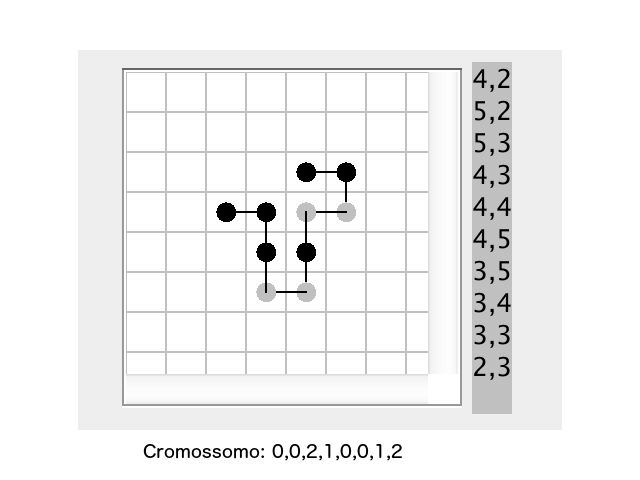
\includegraphics[scale=0.36]{Imagens/DecodedCromossome.png}
	\caption{Cromossomo decodificado que representa uma possível conformação para a cadeia HHPPHPPHHH}
	\label{img:cromossomo}
\end{figure}


\section{Conjunto de Heurísticas de Baixo Nível}

Para ambas as abordagens o mesmo conjunto de heurísticas de baixo nível (operadores de cruzamento/mutação e busca locais) foi selecionado a partir dos estudos anteriores \cite{custodio2014multiple, custodio2004investigation, garza2012locality,benitez2015algoritmo}. O conjunto de heurísticas de baixo nível será descrito abaixo:

 \begin{itemize}
 	
 		\item \textit{Single Point Crossover} (1X): Este operador seleciona, de maneria aleatória, 1 ponto de cruzamento dividindo os indivíduos em 2 partes. Os genes entre as posições selecionadas são trocados entre os pais de modo a gerar dois novos filhos \cite{benitez2015algoritmo}.
 	
 	\item \textit{Two Points Crossover} (2X): Este operador seleciona, de maneria aleatória, 2 pontos de cruzamento dividindo os indivíduos em 3 partes. Os genes entre as posições selecionadas são trocados entre os pais de modo a gerar dois novos filhos \cite{benitez2015algoritmo}, conforme apresentado na figura \ref{fig:twopointscrossover}.
 	
 	
 	\begin{figure}[!htb]
 		\centering
 		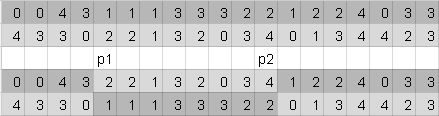
\includegraphics{Imagens/TwoPointsCrossover.png}
 		\caption{Exemplo de aplicação do operador 2x. \\Fonte Autoria Própria}
 		\label{fig:twopointscrossover}
 	\end{figure}
 	
 	
 	
 	
 	\item \textit{Multi Points Crossover} (MPX): Semelhante ao 2X porém com c pontos, baseado na função $c = int(n * 0.1)$, onde $n$ é o tamanho da sequência. O operador MPX é utilizado para promover diversidade estrutural realizando uma mescla randômica entre os pais. Embora, não tão radical quanto o \textit{Uniform  Crossover} \cite{sabar2015automatic}. Um exemplo de aplicação do operador MPX é apresentado na imagem \ref{fig:multipointscrossover}
 	
 	
 	\begin{figure}[!htb]
 		\centering
 		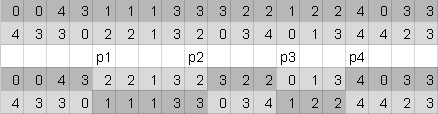
\includegraphics{Imagens/MultiPointsCrossover.png}
 		\caption{Exemplo de aplicação do operador MPX. \\Fonte Autoria Própria}
 		\label{fig:multipointscrossover}
 	\end{figure}
 	\item \textit{Segment Mutation} (SMUT): Altera um número aleatório (5 a 7) de genes consecutivos para direções distintas. Esta heurística introduz grandes mudanças na conformação, e tem uma grande probabilidade de criar colisões. Um mecanismo de reparação simples é aplicado no descendente gerado. A imagem \ref{fig:segmentMutation} apresenta um exemplo da aplicação do SMUT.
 	
 	\begin{figure}[!htb]
 		\centering
 		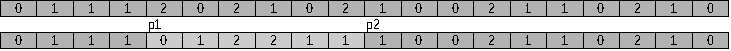
\includegraphics{Imagens/segmentMutation.png}
 		\caption{Exemplo de aplicação do operador SMUT. \\Fonte Autoria Própria}
 		\label{fig:segmentMutation}
 	\end{figure}
 	
 	
 	\item \textit {Exhaustive Search Mutation} (EMUT): Esta heurística seleciona um gene aleatório e testa todas as outras direções possíveis. Manterá a alteração que conseguir aumentar a qualidade da estrutura. O \textit{tradeoff} deste operador é demandar 4 avaliações de \textit{fitness}, há mais que as demais. Esta heurística tem grande potencial de melhorar o \textit{fitness} de uma estrutura. 
 	
 	
 	\item \textit{Local Move Operator} (LM): Esta heurística troca direções entre dois genes aleatórios consecutivos. Existem algumas condições para que esta heurística possa ser executada, por exemplo, as novas direções não podem criar movimentos redundantes. A figura \ref{fig:localMoveOperator} apresenta um exemplo da aplicação do operador LM. 
 	
 	
 	\begin{figure}[!htb]
 		\centering
 		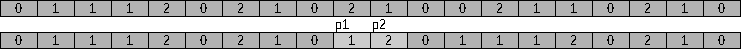
\includegraphics{Imagens/LocalMoveOperator.png}
 		\caption{Exemplo de aplicação do operador LM. \\Fonte Autoria Própria}
 		\label{fig:localMoveOperator}
 	\end{figure}
 	
 	
 	\item \textit{Loop Move Operator} (LPM): Da mesma maneira que a heurística LM, esta heurística troca direções entre dois genes que estão a 5 genes de distância na sequência. A figura  \ref{fig:loopMoveOperator} apresenta um exemplo da aplicação do operador LPM.
 	
 	
 	\begin{figure}[!htb]
 		\centering
 		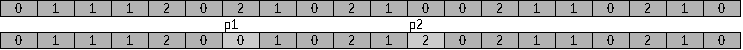
\includegraphics{Imagens/LoopMoveOperator.png}
 		\caption{Exemplo de aplicação do operador LPM. \\Fonte Autoria Própria}
 		\label{fig:loopMoveOperator}
 	\end{figure}
 	
 	\item \textit{Opposite Mutation} (OM): Esta heurística troca as direções, para direção oposta, de uma sequência de genes entre dois genes $(i,j)$ selecionados de maneira aleatória. A direção 0 ($F$) não possui oposta, portanto é mantida. Para exemplificar, suponha esta solução hipotética para uma sequência de 5 aminoácidos: $\{0,1,2,1,2\}$. Ela se tornaria $\{0,2,1,2,1\}$. A figura \ref{fig:oppositeMutation} apresenta um exemplo da aplicação do operador OM.
 	
 	
 	\begin{figure}[!htb]
 		\centering
 		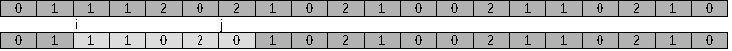
\includegraphics{Imagens/OppositeMutation.png}
 		\caption{Exemplo de aplicação do operador OM. \\Fonte Autoria Própria}
 		\label{fig:oppositeMutation}
 	\end{figure}
 	
 	
 	
 \end{itemize} 



 Este capítulo está divido em duas seções para melhor apresentar ambas as estratégias propostas nesta dissertação. A seção \ref{sec:aemos} apresenta a estratégia multi objetiva onde foi utilizada dois algoritmos evolucionários, do estado da arte de otimização multi objetiva. Já a seção  \ref{sec:eghypdp} irá apresentar o design automático de heurísticas de alto nível para um \textit{framework} hiper heurístico para resolver o PDP.

	



\section{AEMOs aplicados ao PDP}
\label{sec:aeoms}

Esta abordagem utiliza uma modelagem multi-objetiva para PDP baseado no estudo desenvolvido por \cite{gabriel2012algoritmos}. O primeiro objetivo consiste em maximizar a quantidade de contatos topológicos das estruturas de proteínas. Já o segundo  trata de minimizar a máxima distância euclidiana entre os aminoácidos. 

Duas abordagens multi-objetivas foram desenvolvidas neste capítulo, utilizando os AEMOs (NSGAII e IBEA) descritos no capítulo \ref{cap:Referencial Teórico}. A primeira abordagem consistiu em aplicar os algoritmo IBEA and NSGAII utilizando suas versões padrão. Nesta abordagem os operadores genéticos (cruzamento e mutação) são fixos com: \textit{Single Point Crossover (1x)} and \textit{Bit Flip Mutation (BM)}. Esta foi a combinação que obteve os melhores resultados em experimentos preliminares. No caso da segunda abordagem, o IBEA e NSGAII foram modificados com objetivo de aprimorar os resultados em relação às versões padrões. Duas modificações foram propostas e serão descritas abaixo:

 
 \begin{itemize}
 		
		\item \textit Conjunto de heurísticas de baixo nivel: O uso de operadores fixos geralmente não conseguem guiar a busca para regiões promissoras. 
		Com objetivo de aprimorar os AEMOs, . Os operadores que compõem conjunto foram selecionados de estudos anteriores e foram apresentados no início deste capítulo. A cada operação de cruzamento e mutação os operadores são selecionados de maneira aleatória a partir do conjunto. Os operadores são sempre executados independente de probabilidades conforme a versão padrão dos algoritmos. 
	
		
		\item Inicialização via \textit{backtracking}: Tradicionalmente, a população inicial é gerada de maneira aleatória no caso dos algoritmos NSGAII e IBEA. Este tipo de inicialização tem grande potencial de gerar muitas soluções inválidas ao  modelo HP-2D. Soluções que não sejam \textit{self-avoiding walk} (SAW) são consideradas inválidas pois dois ou mais aminoácidos estariam ocupando a mesma posição no espaço. Se a população for integralmente gerada de maneira aleatória os algoritmos de otimização perdem um tempo considerável avaliando soluções inválidas. Para evitar este problema uma estratégia de \textit{backtracking} pode ser utilizada. A estratégia de inicialização com \textit{backtracking} irá começar posicionando o primeiro aminoácido na posição 0,0. Para posicionar o próximo aminoácido, um movimento é selecionado de maneira aleatória. Caso o movimento cause uma colisão, este movimento será marcado como uma má escolha e um novo movimento é selecionado aleatoriamente (do conjunto que restou sem os movimentos marcados como más escolhas). Caso todos os movimentos estejam marcados como má escolha, a estratégia de \textit{backtracking} irá retornar de maneira recursiva para o aminoácido anterior e marcar a escolha em questão como uma má escolha. A estratégia de \textit{backtracking} termina quando gerar uma conformação que não possua colisões. Entretanto, a inicialização via \textit{backtracking} é computacionalmente custosa. Dessa maneira, apenas 20\% da população inicial foi inicializada utilizando esta estratégia.

\end{itemize}

Portanto 4 algoritmos foram implementados (IBEA, NSGAII, M\_IBEA e M\_NSGAII) foram propostos para avaliar a abordagem multi objetiva para o PDP simplificado.


\subsection{Funções Objetivo}


\begin{itemize}
	\item \textbf{Valor de Energia}: Este é o objetivo principal e sua responsabilidade é avaliar o valor de energia associado com as possíveis conformações codificadas pelos cromossomos. O objetivo é minimizar o valor de energia, o qual, é calculado conforme descrito no capítulo \ref{cap:pdp}. Este objetivo guia a busca na direção onde os valores energia associados com as estruturas de proteínas sejam mínimos. Dessa maneira, obtendo conformações mais próximas ao estado nativo das estruturas de proteínas.

    \item \textbf{Distância euclideana entre os resíduos mais distantes}: Este é um objetivo secundário inspirado pelo estudo desenvolvido por \cite{gabriel2012algoritmos}. A motivação por de trás deste objetivo é que estruturas mais compactas tendem a possuir mais contatos hidrofóbicos, oque resultaria em um valor menor de energia. A distância entre os resíduos é calculada utilizando a distância euclidiana.
   
\end{itemize}

Geralmente para avaliar e comparar a performance dos AEMOs, indicadores de qualidade são utilizados. Neste estudo o indicador \textit{hypervolume} foi utilizado. Este indicador considera o volume do espaço de busca dominado pela fronteira conhecida de Pareto obtida por um algoritmo \cite{zitzler2003performance}. Um maior valor de \textit{hypervolume} significa maior qualidade na cobertura do que um algoritmo com valor inferior.

Os 4 algoritmos foram implementados utilizando a arquitetura \textit{open source} disponível no \textit{framework} jMetal. A arquitetura do jMetal é de fácil extensão e possui uma ativa comunidade.


\section{EGHyPDP}
\label{sec:eghypdp}

Esta abordagem é baseada no trabalho desenvolvido por \cite{sabar2015automatic}, o qual  utilizou GEP (\textit{gene expression programming}) com objetivo de gerar, de maneira \textit{online}, os componentes de um \textit{framework} hiper-heurístico para diversos domínios de problemas. Os testes de generalidade realizados, utilizando os 6 domínios providos pelo \textit{framework} hiper-heurístico HyFlex, apresentaram bons resultados em relação às outras estratégias hiper-heurísticas do estado da arte. Nesta proposta pretende-se utilizar EG ao invés de GEP e aplicar ao PDP simplificado utilizando o modelo HP-2D. Da mesma maneira que a abordagem que utilizou  AEMOs a representação de coordenadas relativas descrita na subseção \ref{subsubsection:modeloHP}, será utilizada. Como mencionado anteriormente, um \textit{framework} hiper-heurístico possui dois níveis: alto (\textit{high-level heuristics}) e baixo (\textit{low-level heuristics}). Nesta proposta as heurísticas de alto nível são compostas por: um mecanismo de seleção e um critério de aceitação. Já as heurísticas de baixo nível consistem em um conjunto de heurísticas, selecionadas de estudos anteriores, um mecanismo de memória e uma função de \textit{fitness}. 

\section{Heurísticas de alto nível}
\label{sec:highlevelheuristics}
Esta abordagem  foi desenvolvida para construir de maneria \textit{offline} os componentes de uma heurística de alto nível (mecanismo de seleção e critério de aceitação) para compor um \textit{framework} hiper-heurístico. A figura \ref{fig:proposedFramework} apresenta a estrutura geral do EGHyPDP. 

\begin{figure}[!htb]
	\centering
	\includegraphics[scale=.98]{Imagens/proposedFramework.png}
	\caption{ \textit{Estrutura geral do EGHyPDP.} \\ Fonte: Adaptado de \cite{sabar2015automatic}}
	\label{fig:proposedFramework}
\end{figure}


Heurísticas de alto nível geralmente levam em consideração uma ou mais informações referentes ao histórico das aplicações das heurísticas de baixo nível para tomar suas decisões. Tradicionalmente, informações tais como desempenho (capacidade de melhorar soluções), tempo (desde a última aplicação de uma dada heurística) e intervalo de confiança (no caso de estratégias que utilizam MAB) são utilizadas como base de conhecimento. \cite{sabar2015automatic} propõem a utilização de vários critérios para avaliar as heurísticas de baixo nível. Cada critério irá favorecer a seleção de uma heurística de baixo nível a partir de um aspecto diferente. Por exemplo, algumas heurísticas de baixo nível podem ter bom desempenho apenas no início da busca, enquanto outras podem obter melhores resultados apenas ao final. Estes critérios propostos por \cite{sabar2015automatic} contém estatísticas referente à aplicações das heurísticas de baixo nível e são genéricos o suficiente para serem aplicados ao PDP. Os critérios propostos por Sabar et al. \cite{sabar2015automatic} são detalhados em seguida:


\begin{itemize}
	\item RC (\textit{Reward Credit}): Representa a recompensa que uma determinada heurística de baixo nível deve receber baseado no seu desempenho durante o processo de busca. Quando a i-ésima heurística é aplicada, a melhoria para a solução é computada. O cálculo da melhoria é dado por: $M(i) = (|f1 -f2|/f1) *100$ se $f2$< $f1$, onde $f1$ é a qualidade da solução corrente e $f2$ é a qualidade da solução resultante após a aplicação da i-ésima heurística. 
	A melhoria obtida é salva em uma janela deslizante (FIFO) de tamanho W. O crédito de qualquer heurística de baixo nível é então atribuído como o máximo valor na janela deslizante correspondente. A ideia por trás deste critério é: heurísticas de baixo nível que não são usadas com frequência mas que alteram a solução com grandes melhorias tendem a ter mais preferência do que aquelas que geram pequenas melhorias. Portanto as heurísticas que trazem frequentes, mas pequenas melhorias irão ter menos probabilidade de serem selecionadas.
	\item $C_{best}$: Número de vezes que a i-ésima heurística de baixo nível atualizou a melhor solução conhecida. Este critério favorece as heurísticas de baixo nível que obtiveram êxito em melhorar a melhor solução conhecida até o momento. Este critério é útil para sistematicamente melhorar o atual mínimo local.
	\item $C_{current}$: Número de vezes que a i-ésima heurística de baixo nível atualizou a solução atual. Este critério favorece as heurísticas de baixo nível que obtém êxito em atualizar a solução corrente. Este critério serve para deixar a busca concentrada próxima à solução corrente.
	\item $C_{accept}$: Número de vezes que a solução gerada pela i-ésima heurística de baixo nível foi aceita pelo critério de aceitação. Irá favorecer heurísticas de baixo nível que podem ajudar a escapar de um mínimo local.
	\item $C_{ava}$: A média de melhorias anteriores da i-ésima heurística de baixo nível durante o progresso da busca. Este critério favorece heurísticas de baixo nível que realizaram grandes melhorias em média.
	\item $C_r$: O número de vezes que a i-ésima heurística de baixo nível foi classificada como primeira.  
\end{itemize} 

Da mesma maneira \cite{sabar2015automatic} propõem o uso de dados referentes ao histórico de aplicações das heurísticas de baixo nível para compor critérios de aceitação que irão definir limites para aceitar soluções com qualidade inferior. Dessa forma, um conjunto de fatores também foi proposto e será detalhado em seguida:


\begin{itemize}
	\item Delta: A diferença da qualidade entre a solução corrente e a solução descendente.
	\item PF: A qualidade da solução anterior.
	\item CF: A qualidade da solução atual.
	\item CI: Iteração corrente.
	\item TI: Número de iterações.
\end{itemize}


Utilizando estes dados estatísticos e um conjunto de funções matemáticas simples, tais como soma, subtração, multiplicação e divisão, uma gramática foi desenvolvida para suportar a geração das heurísticas de alto nível. A gramática desenvolvida para gerar mecanismos de seleção e critérios de aceitação é apresentada na Gramática \ref{grammar:proposedGrammar}. 

Para inicializar os dados dos terminais: todas as heurísicas foram executadas uma vez e os dados para cada terminal foi calculado. Toda iteração seguinte irá atualizar os dados dos terminais e essas informações são utilizadas durante a busca.

 \begin{Grammar}
 	\begin{grammar}
 		<hh-selection> ::= <selection-mechanism> <acceptance-criterion> 
 		
 		<selection-mechanism> :==  <selection-terminal>   
 		\alt <selection-mechanism> <math-function> <selection-mechanism> 
 		\alt (<selection-mechanism> <math-function> <selection-mechanism>) 
 		
 		<selection-terminal> :== 
 		RC 
 		| Cbest 
 		| Ccurrent 
 		| Caccept 
 		| Cava 
 		| Cr
 		
 		<math-function> :== + 
 		| - 
 		| * 
 		| \%
 		
 		<acceptance-criterion> ::== <acceptance-terminal> 
 		\alt <acceptance-criterion> <math-function>
 		<acceptance-criterion>
 		\alt (<acceptance-criterion>  <math-function> <acceptance-criterion>) 
 		
 		<acceptance-terminal> :== PF | CF | CI | TI
 		
 		%	<acceptance-function> :== + | - | * | \% | $e^x$
 		
 		
 	\end{grammar}
 	\caption{Gramática definida para gerar  heurísticas de alto nível}
 	\label{grammar:proposedGrammar}
 \end{Grammar}
 
 
  
  O conjunto de funções matemáticas para combinar de diferentes maneiras os dados históricos das aplicações das heurísticas de baixo nível é apresentado abaixo:
  
  \begin{itemize}
  	\item +: Adiciona as duas entradas.
  	\item -: Subtrai a segunda entrada da primeira.
  	\item *: Multiplica as duas entradas.
  	\item \%: Divisão protegida, isto é, se o denominador for 0, o altera para 0,001.
  \end{itemize}
  
  
  Utilizando a Gramática \ref{grammar:proposedGrammar} e vetores de inteiros é possível gerar heurísticas de alto nível. Os conjuntos terminais da gramática apresentam estatísticas sobre as heurísticas de baixo nível e estas são a matéria-prima para a construção dos componentes das heurísticas de alto nível de um \textit{framework} hiper-heurístico. 
  
  

  
  O próximo passo consiste em evoluir uma população de vetores de inteiro utilizando o processo evolutivo descrito na subseção 
  \ref{subsubsection:EvolucaoGramatical}. %A figura BLAH apresenta o processo geral da evolução gramatical proposta.
  
  
  \subsection{Função de \textit{Fitness}}
  \label{sub:funcfitness}
  
  
  	%TODO: escrever na metodologia sobre a funao de fitness escrever uma funcao bunitinha 
  	
 Com objetivo de avaliar os indivíduos gerados durante a busca, uma função de \textit{fitness} foi desenvolvida. A função executa a heurística de alto nível, representada por um dado indivíduo, em 3 instâncias aleatórias de um total de 11 selecionadas dos estudos anteriores. Para cada instância a heuristíca de alto nível foi executada com um tempo máximo de 30 minutos e o retorno é a melhor solução para o PDP simplificado com o modelo HP-2D. O valor de \textit{fitness} associado com a solução retornada é então normalizado entre 0 e 1. O \textit{fitness} de um indivíduo, da EG, consiste na soma das saídas das execuções com cada uma das 3 instâncias. Dessa maneira, o melhor valor possível é 3 e o pior é 0. A razão de executar a heurística de alto nível (indivíduo) com 3 instâncias é que treinar a EG com apenas uma poderia torna as heurísticas geradas muito especializadas na instância utilizada. Portanto 1/4 do número total de instâncias foi utilizado para tentar tonar as heurísticas menos especialistas e mais genéricas. 
 
% 
%\begin{equation}
% 	\sum_{i = 0}^{n}E(c_i)
% \end{equation}
%
%\noindent onde $ c $ é o conjunto de instâncias selecionadas de maneira aleatória no inicio do processo da EGHyPDP, sendo que o tamanho máximo, $ n $ foi definido como três.
 
 
 
   


  
  \subsection{Critério de Parada}
  \label{sub:criterioParada}
  
  Para terminar o processo da EG um número máximo de iterações que não obtêm melhora será utilizado como condição de parada. Note que este critério de parada é referente à parada do processo da EG e não das execuções dos indivíduos dentro do \textit{framework} hiper-heurístico, que ocorrem durante o progresso da EG. 
  
  
  \section{Heurísticas de baixo nível}
  
  Nas heurísticas de baixo nível o EGHyPDP possui 2 componentes principais: um conjunto de heurísticas de baixo nível e um mecanismo de memória.
  
  \subsection{Conjunto de heurísticas de baixo nível}
  O conjunto de heurísticas de baixo nível foi desenvolvido baseado estudos anteriores e foi apresentados no início deste capítulo.
  



\section{Processo geral do EGHyPDP} 

As principais etapas da EGHyPDP proposta serão apresentadas nesta seção.
Inicialmente uma população de indivíduos (heurísticas de alto nível: mecanismos de seleção e critérios de aceitação) é gerada conforme o procedimento que será descrito posteriormente nesta seção. O \textit{fitness} da população é calculado inserindo os indivíduos em um \textit{framework} hiper-heurístico e o executando com 3 instâncias por 30 minutos. E de maneira iterativa selecionar indivíduos pais e aplicar os operadores de cruzamento, \textit{prune}, mutação, e \textit{duplicate} para gerar descendentes. Posteriormente, estes indivíduos são submetidos ao processo de avaliação descrito na subseção \ref{sub:funcfitness}.

%Para avaliar os indivíduos gerados, os seguintes passos são executados:


O processo da EGHyPDP irá parar apenas quando o critério de parada discutido na subseção \ref{sub:criterioParada} for atingido e será retornado o indivíduo (heurística de alto nível) que possuir o maior valor de \textit{fitness}. Também será retornada a solução ao PDP que tiver maior qualidade no mecanismo de memória.



\subsection{Mecanismo de Memória}
\label{sub:MecanismoDeMemoria}

A maioria dos \textit{frameworks} hiper-heurísticos propostos na literatura operam sobre uma única solução \cite{chakhlevitch2008hyperheuristics, burke2013hyper}. Blum et al. \cite{blum2011hybrid} menciona que utilizar uma única solução pode restringir a capacidade de explorar complexos espaços de busca e com alta variância de características. Dessa maneira,  \cite{sabar2015automatic} propôs uma abordagem que utiliza um mecanismo de memória, assim como  \cite{talbi2006cosearch}, o qual contém um conjunto de soluções com alta qualidade e diversificadas, atualizado durante o progresso da busca. Nesta proposta o mecanismo de memória tem a responsabilidade de armazenar soluções para o problema PDP utilizando a representação de coordenadas relativas para o modelo HP-2D. 

\subsubsection{Inicialização do Mecanismo de Memória}

Tradicionalmente algoritmos evolutivos inicializam suas populações iniciais de maneira aleatória, por conta disto  muitas soluções inválidas ao modelo HP, são geradas na inicialização. Isto geralmente  ocasiona perda de tempo de processamento, por conta da grande quantidade de conformações inválidas antes que bons resultados sejam obtidos. Diante disto, \cite{benitez2015algoritmo} propôs uma estratégia especializada de inicialização. A população de seu algoritmo genético, é dividia em duas partes. Uma gerada aleatoriamente, com indivíduos que potencialmente possuem colisões. E uma segunda parte onde todos os indivíduos são livres de colisões. Uma configuração é utilizada para definir a proporção entre as duas partes da população inicial. Para garantir que os indivíduos não possuam colisões, uma estratégia de \textit{backtracking} deve ser utilizada. Nesta abordagem, a mesma estratégia de inicialização via \textit{backtracking }, descrita  na seção \ref{sec:aeoms} foi implementada.





%As possíveis conformações podem ser representadas por um caminho em um grafo orientado estruturado como uma árvore. Consequentemente, cada nó da árvore representa uma solução candidata parcial $c$, desde o primeiro aminoácido até o último sendo considerado. Portanto, um caminho até um nó folha representa uma conformação completa. As arestas do grafo representam o movimento de cada aminoácido relativo a seu predecessor.



\subsubsection{Atualização do Mecanismo de Memória}
Para cada indivíduo (heurística de alto nível) será selecionada de maneira aleatória uma solução do mecanismo de memória e a busca irá iniciar em torno desta solução, quando o \text{framework} hiper-heurístico atingir o seu número máximo de iterações a solução final tem que ser avaliada para verificar sua qualidade e diversidade. A qualidade de uma solução para o PDP utilizando o modelo HP é inversamente proporcional à quantidade de interações entre aminoácidos hidrofóbicos. Portanto a qualidade de uma solução é dada pela quantidade de iterações H-H multiplicada por -1, conforme descrito na subseção \ref{subsubsection:modeloHP}.  As soluções geradas que tiverem a qualidade maior que todas as soluções contidas no mecanismo de memória substituirão a solução que tiver menor similaridade segundo a distância de  \cite{hamming1950error}. Se a qualidade de uma solução gerada não for maior que todas as soluções, mas melhor em relação a um sub-conjunto do mecanismo de memória, esta substituirá a solução que tiver menor qualidade e menor similaridade do sub-conjunto. E por fim se a qualidade da solução gerada for pior que todas contidas no mecanismo de memória, esta é descartada. A similaridade é considerada a fim de manter a diversidade entre as soluções.  



\section{Considerações Finais}
\label{Metodologia:ConsideracoesFinais}

Neste capítulo foram discutidos os principais aspectos relativos à duas estratégias propostas nesta dissertação. Inicialmente, foi discutido sobre a aplicação de AEMOs e em seguida o EGHyPDP foi apresentado. A representação relativa foi utilizada para codificar as soluções para ambas as estratégias. O conjunto de heurísticas de baixo nível, utilizado em ambas abordagens, também foi apresentado. No caso dos AEMOs 4 versões de algoritmos foram apresentadas. As funções objetivas também foram discutidas. Duas adaptacões foram propostas que consistiram em adicionar um conjunto heurísticas de baixo nível para tornar os AEMOs mais adpatativos e a inicialização via \textit{backtracking}. Para aplicar o EGHyPDP com objetivo de gerar heurísticas de alto nível de um \text{framework} hiper-heurístico para o PDP simplicado, uma  gramática foi desenvolvida. Também foi apresentado um conjunto de terminais referente ao histórico das aplicações das heurísticas de baixo nível. Funções matemáticas simples compõem a gramática e combinadas com os dados estatísticos diferentes heurísticas de alto nível foram geradas. Posteriormente, a função de \textit{fitness} avalia estas heurística executando o \textit{framework} composto por tais trés vezes em três instâncias distintas selecionadas de maneira aleatória.
 
 O próximo capítulo apresenta os experimentos realizados afim de avaliar o desempenho das abordagens aqui propostas.



		% proposta
\chapter{Experimentos}
\label{cap:experimentos}

Neste Capítulo serão apresentados  os experimentos para  validar as duas estratégias apresentadas no Capítulo \ref{cap:Metodologia}. 
O conjunto de \textit{benchmark} para avaliar o desempenho dos das abordagens ao PDP simplificado com modelo HP-2D


A partir da revisão bibliográfica foi possível selecionar 11 instâncias dos trabalhos relacionados \cite{unger1993genetic,krasnogor2002multimeme,shmygelska2002ant,shmygelska2003improved,hsu2003growth} para compor um conjunto de \textit{benchmark}. Este conjunto foi utilizado para avaliar ambas estratégias propostas, a Tabela \ref{tab:instancias} apresenta o tamanho, o melhor valor de energia conhecido e a fórmula da sequência de aminoácidos para o modelo HP. Tanto os AEMOs e o EGHyPDP foram submetidos a esse conjunto de instâncias o qual possui diferentes níveis de complexidade e características. Todos os experimentos realizados nesta dissertação foram executados 30 vezes por conta do comportamento estocástico inerente às heurísticas utilizadas. Por conta das múltiplas execuções em casos que forem necessários serão apresentados os valores de média, desvio padrão, minimo e máximo referente as execuções.


Este capítulo esta divido em duas seções para melhor apresentar os resultados obtidos por cada uma das estratégias propostas. A primeira seção descreve os experimentos realizados para avaliar a aplicação de AEMOs para o PDP utilizando o modelo HP-2D. A segunda seção apresenta os experimentos realizados para avaliar a habilidade do EGHyPDP em gerar heurísticas de alto nível para um \textit{framework} hiper heurístico, utilizando um procedimento de EG.



 
\begin{table}[]
	\centering
	\caption{Instâncias de \textit{benchmark} utilizadas nos experimentos.}
	\label{tab:instancias}
	
	\resizebox{\columnwidth}{!}{%
	\begin{tabular}{cccc}
		Instância & Tamanho & \multicolumn{1}{l}{Melhor Valor de Energia} & Fórmula HP                                                                                                                                                                          \\ \hline
	1       & 20      & -9                          & $HPHPPHHPHHPHPHHPPHPH$                                                                                                                                                               \\ \hline
	2       & 24      & -9                          & $HHPPHPPHPPHPPHPPHPPHPPHH $                                                                                                                                                           \\ \hline
		3       & 25      & -8                          & $PPHPPHHP^4HHP^4HHP^4HH$                                                                                                              \\ \hline
		4       & 36      & -14                         & $P^3HHPPHHP^5H^7PPHHP^4HHPPHPP$                                                                                       \\ \hline
		5       & 48      & -23                         & $PPHPPHHPPHHP^5H^{10}P^6HHPPHHPPHPPH^5$                                                                             \\ \hline
		6       & 50      & -21                         & $HHPHPHPHPH^4PHP^3HP^3HP^4HP^3HP^3HPH^4{{PH}}^4H$ \\ \hline
		7       & 60      & -36                         & $PPH^3PH^8P^3H^{10}PHP^3H^{12}P^4H^6PHHPHP$      \\ \hline
		8       & 64      & -42                         & $H^{12}PHPH{{PPHH}}^2PPH{{PPHH}}^2PPH{{PPHH}}^2PPHPHPH^{12}$                          \\ \hline
		9       & 85      & -53                         & $H^4P^4H^{12}P^6H^{12}P^3H^12P^3H^12P^3HP^2H^2P^2H^2P^2HPH$      \\ \hline
		10      & 100     & -48                         & $P^6HPH^2P^5H^3PH^5PH^2P^4H^2P^2H^2PH^5PH^10PH^2PH^7P^11H^7P^2HP^3P^6HPH$         \\ \hline
		11      & 100     & -50                         & $P^3H^2P^2H^4P^2H^3PH^2PH^2PH^4P^8H^6P^2H^6P^9HPH^2PH^11P^2H^3PH^2PHP^2HPH^3P^6H^3$ \\ \hline
	
	\end{tabular}
	}	
\end{table}












\section{Resultados dos AEMOs aplicados ao PDP}

Nesta seção serão apresentados o cojunto de experimentos realizados utilizando a abordagem multi-objetiva com os algoritmos NSGAII e IBEA. Inicialmente, serão apresentadas as configurações utilizadas para os algoritmos. Em seguida, uma comparação entre os resultados de cada algoritmo é apresentada. Por fim, uma comparação com os resultados dos trabalhos relacionados, que tratam o PDP de maneira mono-objetiva, é apresentada.

As configurações utilizadas nos AEMOs foi definida baseada no tamanho das instâncias. Para instâncias menores o tamanho da população e o número máximo de avaliações são menores. Já para as sequências maiores os valores utilizados são superiores. A Tabela \ref{tab:popConfiguration} apresenta para cada instância: o tamanho da instância, o tamanho da população e número máximo de avaliações.

No caso das versões padrão dos algoritmos IBEA e NSGAII as probabilidades de cruzamento e mutação foram configuradas com 0.9 e 0.01 respectivamente. A segunda abordagem não necessita de probabilidades, pois os operadores sempre serão aplicados para gerar novos indivíduos. No caso dos algoritmos IBEA e M\_IBEA a população auxiliar foi mantida em 200 para todas as instâncias.

\begin{table}[!htb]
	\centering
	\caption{Tamanho da população, número máximo de avaliações para cada instância}
	\label{tab:popConfiguration}
	\begin{tabular}{ccccl}
		\hline
		Instância & Tamanho & \begin{tabular}[c]{@{}c@{}}Tamanho  \\ 	População\end{tabular} & \begin{tabular}[c]{@{}c@{}}N Max Avaliações \\ \end{tabular} & \multicolumn{1}{c}{} \\ \hline
		1      & 20   & 100                                                        & 25000                                                      &                      \\ \hline
		2      & 24   & 100                                                        & 25000                                                      &                      \\ \hline
		3      & 25   & 500                                                        & 250000                                                     &                      \\ \hline
		4      & 36   & 500                                                        & 250000                                                     &                      \\ \hline
		5      & 48   & 1000                                                       & 2500000                                                    &                      \\ \hline
		6      & 50   & 1000                                                       & 2500000                                                    &                      \\ \hline
		7      & 60   & 2500                                                       & 2500000                                                    &                      \\ \hline
		8      & 64   & 2500                                                       & 2500000                                                    &                      \\ \hline
		9     &  85   & 2500                                                       & 2500000                                                    &                      \\ \hline
		10     &  100   & 3500                                                       & 3500000                                                    &                      \\ \hline
		11     &  100   & 3500                                                       & 3500000                                                    &                      \\ \hline
	\end{tabular}
\end{table}


Conforme mencionado no Capítulo \ref{cap:Metodologia} o indicador \textit{hypervolume} foi utilizado para comparar o desempenho dos AEMOs. Para cada algoritmo a média e o desvio padrão do \textit{hypervolume}  referente a 30 execuções é apresentada na Tabela \ref{tab:hypervolumeResults}. Os maiores valores estão em negrito e indicam uma maior aproximação da fronteira de Pareto \cite{barr1998economics}.

Observando a Tabela \ref{tab:hypervolumeResults} é possível notar que, exceto para a instância $1$, em todas instâncias o algoritmo M\_IBEA (versão modificado com \textit{backtracking} e o \textit{pool} de operadores) obteve a maior média de \textit{hypervolume}. No caso da instância $1$, o IBEA sem modificações obteve a média mais alta. Também vale mencionar, que quando comparando apenas o NSGAII e o M\_NSGAII, a versão modificada obteve as melhores médias. De maneira geral, os AEMOs com \textit{backtracking} e o \textit{pool} de operadores (M\_IBEA and M\_M_NSGAII) apresentaram uma melhoria considerável em relação aos AEMOs tradicionais. Na Tabela \ref{tab:hypervolumeResults}, as células do M\_IBEA que estão marcados com cinza apresentaram diferença estatística de acordo com o teste de  Kruskal-Wallis \cite{mckight2010kruskal} entre os outros algoritmos (NSGAII, M\_NSGAII e IBEA).


\begin{table}[]
	\centering
	\caption{Resultado de média/desvio padrão dos AEMOs}
	\label{tab:hypervolumeResults}
	\begin{tabular}{|c|c|c|c|c|}
		\hline
		\multirow{2}{*}{Instância} & \multicolumn{4}{c|}{\begin{tabular}[c]{@{}c@{}}\textit{Hypervolume} Média\\ (Desvio padrão)\end{tabular}} \\ \cline{2-5} 
		& NSGAII            & M\_NSGAII         & IBEA                     & M\_IBEA                 \\ \hline
		\multirow{2}{*}{1}      & 0.742827          & 0.720864          & \textbf{0.789712}        & 0.786571       \\
		& (0.106315)        & (0.131351)        & (0.067660)               & (0.099424)              \\ \hline
		\multirow{2}{*}{2}      & 0.680572          & 0.712275          & 0.719960                 & \textbf{0.737086}       \\
		& (0.083445)        & (0.137226)        & (0.080727)               & (0.095299)              \\ \hline
		\multirow{2}{*}{3}      & 0.671171          & 0.709898          & 0.716438                 & \textbf{0.738017}       \\
		& (0.129417)        & (0.124201)        & (0.148112)               & (0.155638)              \\ \hline
		\multirow{2}{*}{4}      & 0.702280          & 0.740153          & 0.751755                 & \textbf{0.785728}       \\
		& (0689832)         & (0.075271)        & (0.092427)               & (0.055607)              \\ \hline
		\multirow{2}{*}{5}      & 0.707654          & 0.758128          & 0.733464                 & \cellcolor[HTML]{C0C0C0}\textbf{0.807637}       \\
		& (0.082611)        & (0.062315)        & (0.128757)               & \cellcolor[HTML]{C0C0C0}(0.039620)              \\ \hline
		\multirow{2}{*}{6}      & 0.667771          & 0.774017          & 0.728699                 & \cellcolor[HTML]{C0C0C0}\textbf{0.821177}       \\
		& (0.132218)        & (0.063231)        & (0.080679)               & \cellcolor[HTML]{C0C0C0}(0.048124)              \\ \hline
		\multirow{2}{*}{7}      & 0.784483          & 0.792843          & 0.801778                 & \textbf{0.810351}       \\
		& (0.063257)        & (0.033062)        & (0.067111)               & (0.054576)              \\ \hline
		\multirow{2}{*}{8}      & 0.677464          & 0.705798          & 0.7450656                & \cellcolor[HTML]{C0C0C0}\textbf{0.811439}       \\
		& (0.041287)        & (0.053048)        & (0.036454)               & \cellcolor[HTML]{C0C0C0}(0.050087)              \\ \hline
		
		
			\multirow{2}{*}{9}      & 0.687454          & 0.710798          & 0.7150656                & \cellcolor[HTML]{C0C0C0}\textbf{0.771439}       \\
			& (0.041287)        & (0.043546)        & (0.026561)               & \cellcolor[HTML]{C0C0C0}(0.044087)              \\ \hline
			  
		  
		  \multirow{2}{*}{10}      & 0.650798          & 0.690891         & 0.7250126                & \cellcolor[HTML]{C0C0C0}\textbf{0.761439}       \\
		  & (0.062157)        & (0.033661)        & (0.031211)               & \cellcolor[HTML]{C0C0C0}(0.013186)              \\ \hline
		  
		  
		  
		   
		   \multirow{2}{*}{11}      & 0.630496          & 0.670812         & 0.713126                & \cellcolor[HTML]{C0C0C0}\textbf{0.752445}       \\
		   & (0.052751)        & (0.031235)        & (0.053422)               & \cellcolor[HTML]{C0C0C0}(0.042326)              \\ \hline
	\end{tabular}
\end{table}


\subsection{Comparação com outras abordagens mono-objetivas}
Esta subseção apresenta a comparação dos resultados obtidos pelas melhores variantes de cada AEMO com outras abordagens mono-objetivas propostas em trabalhos anteriores. Os trabalhos comparados são: EDA \cite{santana2008protein}, GA \cite{unger1993genetic}, MMA \cite{krasnogor2002multimeme}, ACO \cite{shmygelska2002ant},  NewACO \cite{ shmygelska2003improved} e PERM \cite{hsu2003growth}. Todos os trabalhos mencionados tratam-se de abordagens mono-objetivas, considerando apenas o valor de energia referente as estruturas de proteínas. A Tabela \ref{tab:comparison} apresenta os melhores resultados, em termos da energia, pelas versões modificadas dos AEMOs, assim como os melhores resultados obtidos pelos estudos anteriores.




\begin{table}[htb]
	\centering
	\caption{Comparação dos melhores AEMOs com o estudos anteriores do PDP}
	\label{tab:comparison}
	\begin{tabular}{ccccccccc}
		\hline
		Instância                   & M\_IBEA      & M\_NSGAII    & \begin{tabular}[c]{@{}c@{}}EDA \\ 
		
		\end{tabular}           & 
		
		\begin{tabular}[c]{@{}c@{}}GA \\ 
		
		\end{tabular}   
		
		& 	\begin{tabular}[c]{@{}c@{}} MMA \\ 
			  
		\end{tabular}        
		&
		\begin{tabular}[c]{@{}c@{}}  ACO \\ 
			
		\end{tabular} 
		& 
		\begin{tabular}[c]{@{}c@{}}  NewACO\\ 
			
		\end{tabular}
		& 
		\begin{tabular}[c]{@{}c@{}}  PERM\\ 
			 
		\end{tabular}
		\\ \hline
		1                     & \textbf{-9}  & \textbf{-9}  & \textbf{-9}  & \textbf{-9}  & \textbf{-9}  & \textbf{-9}  & \textbf{-9}  & \textbf{-9}  \\ \hline
		2                     & \textbf{-9}  & \textbf{-9}  & \textbf{-9}  & \textbf{-9}  & \textbf{-9}  & \textbf{-9}  & \textbf{-9}  & \textbf{-9}  \\ \hline
		3                     & \textbf{-8}  & \textbf{-8}  & \textbf{-8}  & \textbf{-8}  & \textbf{-8}  & \textbf{-8}  & \textbf{-8}  & \textbf{-8}  \\ \hline
		\multicolumn{1}{c}{4} & \textbf{-14}          & -13          & \textbf{-14} & \textbf{-14} & \textbf{-14} & \textbf{-14} & \textbf{-14} & \textbf{-14} \\ \hline
		\multicolumn{1}{c}{5} & \textbf{-23} & -22          & \textbf{-23} & -22          & -22          & \textbf{-23} & \textbf{-23} & \textbf{-23} \\ \hline
		\multicolumn{1}{c}{6} & \textbf{-21} & \textbf{-21} & \textbf{-21} & \textbf{-21} &              & \textbf{-21} & \textbf{-21} & \textbf{-21} \\ \hline
	
		\multicolumn{1}{c}{7} & -35          & -34          & -35          & -34          &              & -34          & \textbf{-36} & \textbf{-36} \\ \hline
	
	\multicolumn{1}{c}{8}                     & \textbf{-42} & -39          & \textbf{-42} & -37          &              & -32          & \textbf{-42} & -38          \\ \hline
		
		9                    & -49 & -44          & -52 & -37          &              & -32          & -52 & \textbf{-53}          \\ \hline
		
		10                    & -43 & -39          & -47 &          &              &           & -47 & \textbf{-48}          \\ \hline
		
		11                    & -41 & -37          & -48  &          &              &           & -47 & \textbf{-50}          \\ \hline
	\end{tabular}
\end{table}

No caso das instâncias $1$, $2$ e $3$ a versões modificadas dos AEMOs (M\_NSGAII e M\_IBEA) obtiveram os mesmos valores mínimos de energia que os estudos  anteriores considerados nesta comparação. No caso da instância $4$, exceto pelo algoritmo M\_NSGAII, todos os outros atingiram o valor de -14. Já no caso da instância $5$ o algoritmo M\_IBEA e 4 algoritmos mono-objetivo obtiveram o valor ótimo de 23. Entretanto, M\_NSGAII e os demais algoritmos obtiveram um valor inferior de -22.    

Já no caso da instância $6$ todos os algoritmos obtiveram o valor ótimo de -21. Para a instância $7$ o algoritmo M\_IBEA obteve -35 da mesma maneira que o EDA. Entretanto o valor ótimo para sequência $7$ é -36 e foi obtido pelo NewACO e PERM. Para a instância $8$ o algoritmo M\_IBEA obteve o valor ótimo -42 mesmo valor que o EDA  e NewACO. Os demais algoritmos obtiveram valores inferiores. No caso das instâncias 9,10 e 11, as maiores, apenas o algoritmo PERM conseguiu obter os melhores resultados. Estas instâncias são as mais complexas devido ao seu tamanho. Dessa maneira, os algoritmos tendem a ficar presos em mínimos locais. Consequentemente, nestes casos os algoritmos necessitam de mecanismos inteligentes para escapar de mínimos locais e guiar a busca para regiões promissoras.

Após analisar os resultados foi possível constatar que apenas um AEMO, o M\_IBEA conseguiu encontrar os melhores resultados para 7 instâncias de 11. Entretanto, nas instâncias mais complexas seu desempenho é degradado. Já os outros AEMOs propostos não obtiveram resultados expressivos.

\subsection{Conclusão dos experimentos utilizando os AEMOs}

AEMOs são algoritmos evolucionários que visam a otimização de múltiplos objetivos em paralelo. Estes apresentam bons resultados quando aplicados a problemas de várias áreas da ciência.  Nestes experimentos dois AEMOs foram aplicados ao problema PDP utilizando o modelo HP-2D. Duas abordagens multi-objetivas foram apresentadas: a primeira utiliza as versões padrão dos algoritmos IBEA e NSGAII; a segunda abordagem consistiu em modificar o IBEA e NSGAII adicionando a inicialização com \textit{backtrack} e o \textit{pool} de operadores, com objetivo de melhorar os resultados. Dado os resultados se tornou claro que as versões modificadas dos algoritmos tem uma maior habilidade em explorar o espaço de busca quando comparados com as versões padrão.  

Também foi possível verificar que a abordagem multi-objetiva utilizando o NSGAII e o M\_NSGAII também não apresentou resultados satisfatórios, tanto em termos de \textit{hypervolume} como valores de energia,  quando comparado com o IBEA e a versão modificada. Mesmo a versão padrão de IBEA obteve melhores resultados do que ambas as versões do NSGAII. Porém, a versão modificada M\_IBEA apresentou os melhores resultados dentre todos AEMOs propostos. Isto sugere que apenas uma formulação multi-objetiva não é suficiente para atingir bons resultados em termos de energia das estruturas. Com a inicialização via \textit{backtracking}, \textit{pool} de operadores e a maneira sofisticada de explorar o espaço de busca multi-objetivo do IBEA  possibilitaram resultados promissores.

Dado os resultados é indiscutível que o algoritmo M\_IBEA foi capaz de escapar dos mínimos locais em vários os casos, exceto para as instâncias 7,9,10 e 11. Estas instâncias são as mais complexas e muitas propostas não conseguem obter os melhores resultados. Dentre  os trabalhos relacionados apenas o PERM consegue  explorar o espaço de busca o suficiente para encontrar os melhores resultados.

Também vale mencionar que os parâmetros para os algoritmos não foram \textit{tunados} e que existe uma chance de obterem melhores resultados caso um procedimento de \textit{tunning} seja feito.

Os resultados obtidos pelo M\_IBEA abrem um amplo campo de possibilidades para aprofundar formulações multi-objetivas para o problema PDP com o modelo HP-2D ou até mesmo o HP-3D. As descobertas desta dissertação motivam pesquisas adicionais utilizando abordagens multi-objetivas e adição de um \textit{pool} de operadores com objetivo de aprimorar a habilidade de escapar de mínimos locais. No caso de formulações multi-objetiva é possível mencionar que o \textit{design} de abordagens inovadoras como o uso de métricas para avaliar o grau de compactação das conformações de proteínas ou outros métodos que considerem diferentes fatores, podem aprimorar os AEMOs e possibilitar que melhores resultados sejam obtidos.



\section{Resultados obtidos com EGHyPDP}

Nesta seção, serão discutidos  os experimentos conduzidos com objetivo de avaliar o \textit{design} automático de heurísticas de alto nível para um \textit{framework} hiper-heurístico. Este \textit{framework} foi aplicado ao PDP para avaliar seu desempenho. A implementação do EGHyPDP ocorreu durante o período de desenvolvimento desta dissertação. 


Três grupos de experimentos foram desenvolvidos e executados. O primeiro grupo de experimentos tratou apenas de gerar mecanismos de seleção. O segundo grupo foi desenvolvido com objetivo de gerar apenas critérios de aceitação. E por último o terceiro grupo foi desenvolvido com intuito de gerar em paralelo tanto mecanismos de seleção como critérios de aceitação.

O tempo de execução total destes 3 grupos de experimentos foi de 28 dias. Após a execução dos experimentos os resultados obtidos por cada grupo foram comparados entre si. Porém esta comparação não foi suficiente para avaliar a capacidade das heurísticas de alto nível. \cite{misir2012intelligent} nos forneceu o código fonte utilizado em seu estudo e isto possibilitou a execução do GIHH (Generic Intelligent Hyper-heuristic) no contexto do PDP com o modelo HP-2D. O GIHH obteve resultados impressionantes em outros problemas de \textit{benchmark}. Portanto, a comparação dos resultados em relação aos obtidos por uma estratégia hiper heurística (do estado da arte) desenvolvida por um pesquisador foi realizada.   	. 

O primeiro grupo de experimentos denominado, EGHyPDP-1, apenas gerou mecanismos de seleção. O critério de aceitação foi configurado e mantido fixo com uma estratégia que aceita apenas soluções melhores ou iguais \cite{burke2013hyper}. O objetivo deste grupo é avaliar a habilidade da abordagem proposta em gerar mecanismos de seleção utilizando um critério de aceitação fixo.

	O segundo grupo de experimentos, EGHyPDP-2, consistiu em gerar apenas critérios de aceitação. O mecanismo de seleção foi configurado e mantido fixo utilizando o melhor mecanismos de seleção gerado pelo experimento EGHyPDP-1. Consequentemente, este experimento depende da saída do primeiro grupo. O objetivo deste experimento é avaliar a qualidade dos critérios de aceitação gerados, separadamente do mecanismo de seleção o qual foi mantido fixo.
	
	O terceiro grupo de experimentos,  EGHyPDP-3, foi desenvolvido para gerar tanto mecanismos de seleção e critérios de aceitação ao mesmo tempo. Este grupo avalia a habilidade em gerar mecanismos de seleção em conjunto com critérios de aceitação. Diferentemente do grupo EGHyPDP-2  , este grupo não depende de nenhuma saída dos experimentos anteriores.


	Para cada grupo de experimentos a fase de treino consistiu em executar o processo da EG utilizando a função de \textit{fitness} descrita no Capítulo \ref{cap:Metodologia}. Na fase de validação o melhor mecanismo de seleção e o melhor critério de aceitação obtidos foram  executados utilizando todas as 11 instâncias descritas na Tabela \ref{tab:instancias}. 
	

	
	\subsection{Resultados obtidos com EGHyPDP-1}
	\label{subsection:gehypdp1results}
	
	O melhor indivíduo (mecanismo de seleção gerado e critério de aceitação melhor ou igual) encontrado no experimento EGHyPSP-1 é apresentado na Equação \ref{eq:bestSelectionMechanism}
	
	\begin{equation}
	\label{eq:bestSelectionMechanism}
	RC * Ccurrent * Cava -Cr.
	\end{equation}
	

	
	Este mecanismo de seleção, juntamente com o critério de aceitação (melhor ou igual) foi executado novamente por 30 vezes com um tempo limite de 30 minutos em cada execução, porém utilizando todas as 11 instâncias disponíveis. A Tabela  \ref{tab:gexp1best} apresenta os resultados de média, desvio padrão, mínimo e máximo das execuções do melhor indivíduo apresentado na Equação \ref{eq:bestSelectionMechanism}. A última linha denota o melhor valor de energia conhecido para cada instância. Os valores destacados com negrito representam os melhores valor conhecido para determinada instância. É possível notar analisando as duas últimas linhas, que exceto para as instâncias 7,9,10 e 11, todas as outras instâncias, o indivíduo gerado conseguiu obter os melhores valores conhecidos. Dessa maneira, é possível observar que quando o tamanho das instâncias aumentam a qualidade dos resultados obtidos degrada.
	

	\begin{table}[]
		\centering
		\caption{Resultados da execução do melhor indivíduo encontrado pelo grupo de experimento EGHyPDP-1}
		\label{tab:gexp1best}
		\resizebox{\columnwidth}{!}{%
			\begin{tabular}{cccccccccccc}
				Instância  & 1   & 2    & 3   & 4    & 5    & 6   & 7   & 8    & 9    & 10   & 11   \\ \hline
				Média   & -8.1 & -7.6 & -6.7 & -11.9 & -17.4 & -16  & -30  & -28.3 & -40.1 & -35.6 & -35.9 \\ \hline
				Desvio Padrão & 0.3 & 0.5  & 0.5 & 0.7  & 1    & 1.4 & 1.7 & 2    & 2.7  & 2.1  & 2.9  \\ \hline
				Máximo   & -8   & -7    & -5   & -11   & -15   & -13  & -25  & -23   & -34   & -32   & -27   \\ \hline
				Mínimo   & \textbf{-9}   & \textbf{-9}    & \textbf{-8}   & \textbf{-14}   & \textbf{-23}   & \textbf{-21}  & -33  & \textbf{-42}   & -46   & -40   & -41   \\ \hline
				Melhor Valor de Energia   & \textbf{-9} & \textbf{-9} & \textbf{-8} & \textbf{-14} & \textbf{-23} & \textbf{-21} & \textbf{-36} & \textbf{-42} & \textbf{-53} & \textbf{-48} & \textbf{-50}  
			\end{tabular}
		}
	\end{table}
	
	\subsection{Resultados obtidos com EGHyPDP-2}
	O melhor indivíduo (mecanismo de seleção fixo e critério de aceitação gerado) encontrado no grupo de experimento EGHyPDP-2 é apresentado na Equação \ref{eq:bestAcceptanceCriteria}. O mecanismo de seleção utilizado foi o mesmo apresentado na Equação \ref{eq:bestSelectionMechanism}. A razão por usar este mecanismo de seleção foi: os resultados obtidos pelo melhor indivíduo da execução do EGHyPDP-1 se apresentaram promissores e o objetivo era gerar um um bom critério de aceitação combinado com um mecanismo de seleção que funcione bem.
	 
	 \begin{equation}
	 \label{eq:bestAcceptanceCriteria}
	( ( TI / Delta ) / ( ( Delta * ( ( TI / Delta ) / CI ) * Delta / Delta * TI ) - CI ) )
	 \end{equation}
		 
	Este critério de aceitação, juntamente com o melhor mecanismo de seleção gerado pelo EGHyPDP-1, foram executados 30 vezes com um tempo máximo de 30 minutos utilizando as 11 instâncias disponíveis. A Tabela \ref{tab:gexp2best}  apresenta os resultados obtidos. Novamente, observando as duas ultimas linhas é possível verificar que em apenas em duas instâncias os melhores valores foram encontrados. Dessa maneira, é fácil notar que os resultados apresentados na Subseção \ref{subsection:gehypdp1results} obtiveram éxito em encontrar, para mais instâncias,  os melhores valores conhecidos. Vale mencionar, que o melhor mecanismo de seleção encontrado combinado com um critério de aceitação melhor ou igual apresentou melhores resultados do que quando combinado com o melhor critério de aceitação gerado. 


	
	\begin{table}[]
		\centering
		\caption{Resultados da execução do melhor indivíduo encontrado no grupo de experimento EGHyPDP-2}
		\label{tab:gexp2best}
		\resizebox{\columnwidth}{!}{%
			\begin{tabular}{cccccccccccc}
				Instância  & 1   & 2   & 3   & 4    & 5    & 6    & 7   & 8    & 9    & 10   & 11  \\ \hline
				Média   & -8   & -7.6 & -6.7 & -10.1 & -14.8 & -14.7 & -27  & -25.7 & -38.3 & -32.8 & -30 \\ \hline
				Desvio Padrão & 0.6 & 0.4 & 0.6 & 0.7  & 1.5  & 1.4  & 2.0 & 2.5  & 3.3  & 3.7  & 3.4 \\ \hline
				Máximo   & -7   & -7   & -5   & -8    & -12   & -12   & -23  & -22   & -31   & -26   & -24  \\ \hline
				Mínimo   & \textbf{-9}   & -8   & \textbf{-8}   & -11   & -17   & -18   & -31  & -31   & -44   & -40   & -37  \\ \hline
				Melhor Valor de Energia   & \textbf{-9} & \textbf{-9} & \textbf{-8} & \textbf{-14} & \textbf{-23} & \textbf{-21} & \textbf{-36} & \textbf{-42} & \textbf{-53} & \textbf{-48} & \textbf{-50}
			\end{tabular}
		}
	\end{table}
	
	\subsection{Resultados obtidos com EGHyPDP-3}
	
	O melhor indivíduo gerado pelo grupo de experimento EGHyPDP-3 é composto por um mecanismo de seleção e um critério de aceitação. As Equações \ref{eq:bestSelectionMechanismWithAccept} e \ref{eq:bestSelectionMechanismWithAccept2} apresentam respectivamente o mecanismo de seleção e o critério de aceitação gerados.
	
	
	\begin{equation}
	\label{eq:bestSelectionMechanismWithAccept}
	( ( ( ( ( Caccept / RC ) * Cr / Caccept ) / RC * Cr ) / Caccept / RC ) * Cr ) / Caccept 
	\end{equation}
	
	
	\begin{equation}
	\label{eq:bestSelectionMechanismWithAccept2}
( ( ( ( ( CI / PF ) * Delta / CI ) / PF * Delta ) / CI / PF ) * Delta ) / CI
	\end{equation}
	
	
	A Tabela \ref{bestGExp3} apresenta os resultados da execução do mecanismo de seleção e do critério de aceitação gerados pelo grupo de experimentos EGHyPDP-3. Da mesma maneira, consistiram em 30 execuções com tempo máximo de 30 minutos. O valores destacados com negrito são os casos que o indivíduo alcançou os melhores valores conhecidos. É possível observar que apenas em dois casos isto ocorreu nas menores instâncias, entre 20 a 25 aminoácidos. Estas sequências são extremamente triviais levando apenas minutos para um  algoritmo genético encontrar as melhores soluções conhecidas. Dessa forma, é possível concluir que a geração de ambas as estratégias neste contexto não apresentou bons resultados. 
	
	\begin{table}[]
		\centering
		\caption{Resultados da execução do melhor indivíduo encontrado no grupo de experimento EGHyPDP-3}
		\label{bestGExp3}
		\resizebox{\columnwidth}{!}{%
			\begin{tabular}{cccccccccccc}
				Instância  & 1   & 2   & 3   & 4   & 5    & 6    & 7   & 8    & 9    & 10  & 11   \\ \hline
				Média  & -7.6 & -7.0 & -5.7 & -9.7 & -13.8 & -12.7 & -24  & -24.2 & -31.6 & -27  & -26.4 \\ \hline
				Desvio Padrão & 0.6 & 0.7 & 0.8 & 0.9 & 1.3  & 0.9  & 1.1 & 1.6  & 1.7  & 1.7 & 2    \\ \hline
				Minímo   & -7   & -6   & -4   & -7   & -12   & -11   & -21  & -21   & -29   & -24  & -24   \\ \hline
				Máximo   & \textbf{-9}   &  -8  & \textbf{-8}   & -11  & -18   & -15   & -26  & -28   & -37   & -31  & -31   \\ \hline
				Melhor Valor de Energia   & \textbf{-9} & \textbf{-9} & \textbf{-8} & \textbf{-14} & \textbf{-23} & \textbf{-21} & \textbf{-36} & \textbf{-42} & \textbf{-53} & \textbf{-48} & \textbf{-50}
			\end{tabular}
		}
	\end{table}
	
	Após estes experimentos foi concluído que apenas a geração de mecanismos de seleção apresentou algum potencial. Os melhores resultados conhecidos foram obtidos em 7 instâncias de um total de 11, utilizando o melhor mecanismo de seleção encontrado. No caso dos critérios de aceitação os resultados não foram como esperados. A hipótese inicial era que combinadas as estratégias de seleção e aceitação esta se complementariam. Dessa maneira, possibilitando que o \textit{framework} hiper heurístico pudesse explorar de maneira adequada o espaço de busca. Apesar do resultado promissor obtido, gerando apenas mecanismos de seleção, é possível notar a perca de desempenho em instâncias maiores (64 a 100 aminoácidos). É questionável: se a falta de um critério de aceitação, melhor do que aceitar apenas soluções melhores ou iguais, pudesse guiar a busca afim de escapar dos mínimos locais. 

	
	
	\subsection{Comparação com \textit{framework} hiper heurístico GIHH}
	
	Com objetivo de comparar a melhor heurística de alto nível obtida pelo grupo de experimentos EGHyPDP-1 uma comparação com o \textit{framework} GIHH proposta por \cite{misir2012intelligent} foi realizada. O GIHH obteve os melhores resultados para 6  domínios distintos de problemas contidos no \textit{framework} HyFlex \cite{ochoa2012hyflex}. Misir disponibilizou o código fonte do GIHH e em seguida foram executados experimentos utilizando o problema PDP com o modelo HP-2D.
	
	A Tabela \ref{tab:gihhandbhlh} apresenta os melhores resultados encontrados pelos experimentos realizados com EGHyPDP, os resultados da execução do GIHH e por fim o melhor valor de energia conhecido. Os valores destacados com negrito são os melhores conhecidos. Tanto o EGHyPDP e o GIHH foram executados por 30 minutos. É possível verificar que em 7 instâncias de um total de 11 o EGHyPDP obteve os melhores valores conhecidos. Já o GIHH conseguiu obter os melhores valores apenas em 5 instâncias. Entretanto, se observamos as instâncias 7,9,10 e 11 o GIHH obteve valores mais próximos dos melhores do que o EGHyPDP. Dessa maneira, é possível afirmar que nas instâncias mais complexas o GIHH consegue chegar mais próximo dos melhores resultados conhecidos. No entanto, o EGHyPDP conseguiu encontrar os melhores valores em mais instâncias do que o GIHH. 
	
	\begin{table}[]
		\centering
		\caption{Os melhores resultados conhecidos e resultados encontrados com o EGHyPDP e GIHH.}
		\label{tab:gihhandbhlh}
		\begin{tabular}{cccccccccccc}
			Instância         & 1 & 2 & 3 & 4  & 5  & 6  & 7  & 8  & 9  & 10 & 11 \\ \hline
			EGHyPDP  & \textbf{-9}   & \textbf{-9}    & \textbf{-8}   & \textbf{-14}   & \textbf{-23}   & \textbf{-21}  & -33  & \textbf{-42}   & -46   & -40   & -41   \\ \hline
			GIHH   & \textbf{-9} & \textbf{-9} & \textbf{-8} & \textbf{-14} & -22 & \textbf{-21} & -35 & -37 & -49 & -43 & -45 \\ \hline
			Melhor Valor de Energia   & \textbf{-9} & \textbf{-9} & \textbf{-8} & \textbf{-14} & \textbf{-23} & \textbf{-21} & \textbf{-36} & \textbf{-42} & \textbf{-53} & \textbf{-48} & \textbf{-50}
		\end{tabular}
	\end{table}
	
	
	\subsection{Discussão}
	O EGHyPDP obteve êxito em gerar um mecanismo de seleção, que combinado com um critério de aceitação que aceita soluções melhores ou iguais, obteve os melhores resultados em 7 instâncias. Entretanto, nas instâncias mais complexas os resultados obtidos são bem inferiores em relação aos melhores valores conhecidos. Também foi constatado que o EGHyPDP conseguiu gerar pelo menos um bom mecanismo de seleção, já no caso dos critérios de aceitação gerados nenhum apresentou bons resultados. Um novo experimento foi realizado para avaliar o comportamento dos critérios de aceitação. Este experimento consistiu em selecionar de maneira aleatória 10 indivíduos gerados pelo experimento EGHyPDP-2 e executá-los novamente para analisar o comportamento de cada um dos 10 critérios de aceitação.
	De 10 indivíduos 7, estavam  aceitando apenas soluções melhores ou iguais, da mesma maneira que o critério fixo que foi utilizado no primeiro experimento EGHyPDP-1. A única diferença entre os indivíduos gerados e o critério fixo: é que os indivíduos são mais lentos que o fixo pois é necessário executar uma expressão aritmética enquanto com o critério fixo, um simples $if$ é avaliado. Mas com respeito ao comportamento os critérios de aceitação são iguais. Outros 2 indivíduos dos 10 selecionados estavam aceitando qualquer solução pior do que a solução corrente da mesma maneira que o critério "todos movimentos" descrito por \cite{burke2013hyper}. Finalmente, um indivíduo não estava aceitando nunca soluções piores da mesma maneira que o critério "apenas melhorias"        
	 \cite{burke2013hyper}.
	
	Estes experimentos mostraram que o EGHyPDP conseguiu várias vezes gerar um critério de aceitação com exatamente o mesmo comportamento que critérios de aceitação desenvolvidos por pesquisadores. Entretanto, estes critérios são muito simples e não são suficientes para possibilitar que a busca não fique travada em mínimos locais. Levando em consideração que os experimentos envolvendo geração de critérios de aceitação (EGHyPDP-2 e EGHyPDP-3) não obtiveram resultados competitivos. 
	
	
	\subsection{Conclusão dos experimentos utilizando o EGHyPDP}
	
	Esta seção apresentou os experimentos realizados com EGHyPDP, uma ferramenta automática para gerar heurísticas de alto nível para um \textit{framework} hiper heurístico para resolver o problema PDP com o modelo HP-2D. O PDP é um problema muito desafiador com uma grande quantidade de mínimos locais e um espaço de busca complexo. 
	
		Muitos estudos exploraram o PDP com modelos simplificados, tais como modelo HP-2D, utilizando métodos heurísticos. Embora, é comum que estratégias heurísticas não consigam obter os melhores resultados conhecidos no caso das maiores instâncias. Geralmente, os \textit{frameworks} hiper heurísticos se adaptam bem a este tipo de contexto complexo. Consequentemente, o objetivo desta abordagem foi gerar mecanismos de seleção e critérios de aceitação, através de um processo de evolução gramatical, de um \textit{framework} hiper heurístico. Tal \textit{framework} foi utilizado para resolver o PDP utilizando o modelo HP-2D. O desempenho e comportamento das heurísticas de alto nível geradas foi avaliado executando o \textit{framework} utilizando um conjunto de 11 instâncias. 
		Trés grupos de experimentos foram desenvolvidos: o primeiro grupo apenas gerou mecanismos de seleção e utilizou um critério de aceitação "melhor ou igual"; o segundo gerou apenas critérios de aceitação. E no caso do mecanismo de seleção foi utilizado o melhor gerado pelo primeiro grupo; O terceiro e último grupo gerou tanto mecanismos de seleção e critérios de aceitação em paralelo. Os resultados obtidos pelos experimentos demonstram que a melhor heurística de alto nível foi encontrada no primeiro grupo. Já os resultados obtidos com o segundo e terceiro grupo não são expressivos. Analisando, o melhor resultado obtido pelo primeiro experimento (um mecanismo de seleção e o critério de aceitação "melhor ou igual") é possível notar que de 11 instâncias em 7 casos foram encontrados os melhores resultados conhecidos. Entretanto, nas maiores instâncias (7,9,10 e 11) os resultados foram inferiores aos melhores conhecidos. 
		O melhor indivíduo gerado também foi comparado com o GIHH, um \textit{framework} hiper heurístico do estado da arte, os resultados obtidos por ambos são ligeiramente próximos. Em 5 instâncias o GIHH conseguiu obter os melhores resultados conhecidos. No caso da instâncias 7,9,10 e 11 o GIHH nao conseguiu encontrar os melhores resultados, mas encontrou resultados supeiores ao EGHyPDP. Isto demonstra que é possível automatizar o \textit{design} de heurísticas de alto nível. E obter resultados próximos aos de uma estratégia hiper heurística com capacidade de obter bons resultados, em outros domínios de problema.
		
		Outra constatação deste estudo foi o comportamento do critérios de aceitação gerados. Foi notado que uma parte dos critérios de aceitação gerados se comportavam da mesma maneira que o critério "melhor ou igual". Também foram gerados critérios que sempre aceitam e que nunca aceitam soluções piores, da mesma maneira que os critérios "todos os movimentos" e "apenas melhorias" respectivamente. Dessa forma, foi possível constatar que os critérios gerados se comportam da mesma maneira que alguns critérios simples, mas que foram desenvolvidos por cientistas. Entretanto, o EGHyPDP não foi capaz de gerar critérios de aceitação que possibilitassem escapar dos mínimos locais de um espaço de busca complexo como o do PDP.

	
	
		% experimentação e validação
\chapter{Conclusão}


Nesta dissertação foram apresentadas duas abordagens heurísticas para o problema PDP utilizando o modelo simplificado HP-2D. 

A primeira abordagem consistiu em uma formulação multi objetiva para o PDP. Um novo objetivo foi adicionado o qual avalia o grau de compactação das estruturas de proteínas. Dessa maneira, considerando o valor da energia e o quão compacta uma dada estrutura é. AEMOs foram utilizados para explorar o espaço de busca no contexto multi objetivo. Os algoritmos utilizados foram o NSGAII \cite{deb2002} e o IBEA \cite{zitzler2004indicator}. Uma versão modificada desses algoritmos, com objetivo de obter melhores resultados, também foi proposta. Os algoritmos M\_NSGAII e o M\_IBEA são versões adaptadas utilizando uma inicialização via \textit{backtracking}  e um \textit{pool} de operadores. Portanto, 4 versões de AEMOs foram utilizadas para tentar resolver o PDP com o modelo HP-2D. Apenas a versão M\_IBEA conseguiu obter resultados expressivos em 7 instâncias de 11. Isto, demonstra que apenas a formulação multi objetiva não é suficiente para explorar o espaço de busca de maneira adequada.  


A segunda abordagem, denominada EGHyPDP, consistiu em gerar as heurísticas de alto nível para um \textit{framework} hiper heurístico, para o PDP utilizando o modelo HP-2D, através da evolução gramatical. Trés grupos de experimentos foram definidos o primeiro gerando apenas mecanismos de seleção; o segundo gerando apenas critérios de aceitação e o terceiro gerando ambos em paralelo. Analisando os resultados obtidos por cada grupo de experimento foi possível perceber que apenas o primeiro grupo de experimentos conseguiu obter resultados expressivos para 7 instâncias de 11. Os outros dois grupos de experimentos conseguiram obter bons resultados apenas para duas instâncias. Dessa maneira, demostrando que os critérios de aceitação gerados não são suficientes para guiar a busca para regiões promissoras. 

Infelizmente nenhuma das abordagens propostas nesta dissertação conseguiu obter os melhores resultados conhecidos para as maiores instâncias. Contudo, ambas as abordagens conseguiram obter bons resultados para 7 instâncias. Tanto o algoritmo M\_IBEA e a melhor heurística de alto nível gerada pelo EGHyPDP obtiveram os melhores resultados nas mesmas instâncias. Já nas instâncias mais complexas, nas quais não foi possível encontrar o melhor resultado conhecido, o M\_IBEA obteve resultados superiores ao EGHyPDP. Porém com diferença estatística segundo o teste de Kruskal-Wallis em apenas uma instância.

O PDP é um problema, em aberto,  extremamente desafiador por conta da enorme quantidade de possíveis soluções contidas no espaço de busca. Dessa maneira,  motivando muitos pesquisadores buscarem métodos mais elegantes e robustos para que estratégias heurísticas não fiquem per .



		% conclusão

%=====================================================

% Estilos de bibliografia recomendados (só descomentar um estilo!)
\bibliographystyle{apalike-ptbr}	% [Maziero et al., 2006]
%\bibliographystyle{plain}		% [1], [1, 2]

% base de bibliografia (BibTeX)
\bibliography{refs}
%\bibliography{ref1, ref2, ref3} % se tiver mais de um arquivo BibTeX

%=====================================================

% apêndices
\appendix
\chapter{Exemplo de anexo}

%=====================================================

Os apêndices são uma extensão do texto, destacados deste para evitar descontinuidade na sequência lógica ou alongamento excessivo de determinado assunto ou tópico secundário dentro dos capítulos da dissertação ou da tese. São contribuições que servem para esclarecer, complementar, provar ou confirmar as ideias apresentadas no texto dos capítulos e que são importantes para a compreensão dos mesmos.

Todos os apêndices devem vir após as referências bibliográficas e devem ser enumerados por letras maiúsculas (A, B, C, ...).

%=====================================================

\section{Uma Seção}

\lipsum[20-23]

%=====================================================

\subsection{Uma sub-Seção}

\lipsum[30-33]

%=====================================================


\end{document}

%=====================================================
